\documentclass[a4paper,12pt]{report}

\usepackage{ucs}
\usepackage[utf8]{inputenc}
\usepackage{amsmath}
\usepackage[italian]{babel}
\usepackage{fontenc}
\usepackage{graphicx}
\usepackage{textgreek}
\usepackage{subcaption}
\usepackage{amsthm}
\usepackage{hyperref}
\usepackage{newlfont}
\usepackage{color}


\textwidth=450pt\oddsidemargin=0pt


\begin{document}

\begin{titlepage}
%
%
% UNA VOLTA FATTE LE DOVUTE MODIFICHE SOSTITUIRE "RED" CON "BLACK" NEI COMANDI \textcolor
%
%
\begin{center}
{{\Large{\textsc{Alma Mater Studiorum $\cdot$ Universit\`a di Bologna}}}} 
\rule[0.1cm]{15.8cm}{0.1mm}
\rule[0.5cm]{15.8cm}{0.6mm}
\\\vspace{3mm}

{\small{\bf Scuola di Scienze \\ 
Dipartimento di Fisica e Astronomia\\
Corso di Laurea in Fisica}}

\end{center}

\vspace{23mm}

\begin{center}\textcolor{black}{
%
% INSERIRE IL TITOLO DELLA TESI
%
{\LARGE{\bf MAGNETIC RESONANCE FINGERPRINTING CON RETI NEURALI A VALORI COMPLESSI}}\\
}\end{center}

\vspace{50mm} \par \noindent

\begin{minipage}[t]{0.47\textwidth}
%
% INSERIRE IL NOME DEL RELATORE CON IL RELATIVO TITOLO DI DOTTORE O PROFESSORE
%
{\large{\bf Relatore: \vspace{2mm}\\\textcolor{black}{
Dott. Enrico Giampieri}\\\\}}
%
% INSERIRE IL NOME DEL CORRELATORE CON IL RELATIVO TITOLO DI DOTTORE O PROFESSORE
%
% SE NON AVETE UN CORRELATORE CANCELLATE LE PROSSIME 3 RIGHE
\end{minipage}
%
\hfill
%
\begin{minipage}[t]{0.47\textwidth}\raggedleft \textcolor{black}{
{\large{\bf Presentata da:
\vspace{2mm}\\
%
% INSERIRE IL NOME DEL CANDIDATO
%
Davide Sangiorgi}}}
\end{minipage}

\vspace{40mm}

\begin{center}
%
% INSERIRE L'ANNO ACCADEMICO
%
Anno Accademico \textcolor{black}{ 2018/2019}
\end{center}

\end{titlepage}






 \chapter*{Abstract}
 
 In questo documento cerco un metodo per migliorare le prestazioni del MRF (Magnetic Resonance Fingerprinting), una tecnica di risonanza magnetica quantitativa. 
 Il problema \'e quello di diminuire il tempo di calcolo necessario per determinare i parametri tissutali relativi alla risonanza magnetica effettuata. 
 Il metodo proposto \'e quello dell'utilizzo di reti neurali a valori complessi con input il segnale di risonanza magnetica e con output i valori relativi ai parametri che si vogliono studiare. 
 
 Dopo aver chiarito il concetto di risonanza magnetica, di MRF ed i problemi ad essi associati, introduco le reti neurali, l'architettura, la dinamica e l'apprendimento relativi ad esse. 
 Discuto di seguito i problemi relativi all'introduzione dei numeri complessi nel modello di rete neurale e anche i vantaggi che le reti neurali a valori complessi possono portare, non solo rispetto ai metodi tradizionali, ma anche rispetto a reti neurali a valori reali.
 
 Analizzo inoltre delle tecniche utili a migliorare la generalizzazione e rendere le reti neurali a valori complessi una soluzione ancora pi\'u concreta. 
 Studio quindi i miglioramenti introdotti dagli ensemble di reti neurali e dall'applicazione di funzioni d'attivazione stocastiche, che introducono del rumore gaussiano all'interno del modello.
 
 \chapter*{Risonanza magnetica}
 
 L'imaging da risonanza magnetica (MRI) \'e una tecnica utilizzata principalmente in campo medico per produrre immagini di sezioni del corpo umano.
 La MRI \'e basata sui principi della risonanza magnetica nucleare (NMR), una tecnica spettroscopica utilizzata per ottenere informazioni di tipo microscopico, chimico e fisico sulle molecole.
 La MRI \'e nata inizialmente come tecnica di imaging tomografico, cio\'e capace di produrre l'immagine di un sottile strato del corpo umano a partire dal segnale NMR.
 Ciascuna sezione \'e composta di vari elementi tridimensionali detti voxel, il cui volume \'e di circa 3 mm3. 
 L'immagine di risonanza magnetica di una sezione risulter\'a composta da un insieme di elementi bidimensionali chiamati pixel, la cui intensit\'a \'e proporzionale all'intensit\'a del segnale NMR del voxel corrispondente.
 
 Il segnale di risonanza magnetica \'e generato dalla rotazione del vettore magnetizzazione dei protoni, in particolare dei protoni dell'idrogeno che compone l' $\mbox{H}_2\mbox{o}$, molecola comune negli organismi viventi. 
 Normalmente i vettori magnetizzazione sono orientati in maniera casuale, ma se sottoposti a campo magnetico esterno stazionario $B_0$, vengono sottoposti allo stesso momento torcente.
 All'equilibrio, il vettore di magnetizzazione risultante \'e posizionato lungo la direzione del campo magnetico statico $B_0$ ed \'e chiamato magnetizzazione all'equilibrio $M_0$. 
 In questa configurazione, la componente Z del vettore di magnetizzazione $M_Z$ \'e uguale a $M_0$. 
 $M_Z$ \'e conosciuta come magnetizzazione longitudinale. 
 Inoltre, sempre per effetto di $B_0$, l'asse di ciascun protone precede attorno alla direzione di $B_0$ con frequenza che \'e caratteristica di ogni elemento atomico e viene denominata frequenza di $Larmor$.
 
 I protoni utilizzati per produrre immagini RM sono quelli dell'idrogeno che, naturalmente, abbondano nei tessuti viventi, in particolare per via delle molecole di acqua.
 Per mettere in risonanza i protoni dell'idrogeno si invia un'onda radio con frequenza pari alla frequenza di Larmor per l'idrogeno.
 Inviando l'impulso di radiofrequenza (RF) si determina la sincronizzazione dei protoni nella stessa fase di precessione generando un vettore di magnetizzazione trasversale, che ruota nel piano xy.
 Una volta cessato l'impulso RF si verifica la progressiva desincronizzazione della precessione dei protoni, con conseguente decadimento della magnetizzazione trasversale ed il ritorno al livello energetico inferiore da parte dei protoni che avevano subito l'inversione 180.
 In ambedue i casi si verifica il fenomeno chiamato rilassamento, durante il quale si generano impulsi (dati dall'oscillazione della magnetizzazione) misurabili tramite la bobina rice-trasmittente (la stessa bobina che in precedenza ha generato l'impulso RF).
 Il rilassamento avviene con due costanti di tempo distinte.
 Il tempo di rilassamento spin-reticolo T1 \'e relativo al ritorno all'equilibrio della magnetizzazione longitudinale. 
 L'equazione che descrive questo fenomeno in funzione del tempo t \'e:
 \begin{equation}
  M_Z = M_0 ( 1 - e^{-t/T_1} )
 \end{equation}
 Se il vettore di magnetizzazione ha subito un impulso RF 180, gradualmente ritorner\'a alla sua posizione di equilibrio sull'asse +Z ad una velocit\'a regolata dal T1, seguendo l'andamento:
 \begin{equation}
  M_Z = M_0 ( 1 - 2e^{-t/T_1} )
 \end{equation}
 Dopo l'impulso RF la componente della magnetizzazione sul piano xy comincia a perdere fase poich\'e ognuno dei pacchetti di spin che la costituiscono \'e sottoposto ad un campo magnetico leggermente diverso e ruota ad una propria frequenza di Larmor. 
 Pi\'u trascorre il tempo, maggiore \'e la differenza di fase e minore la componente sul piano xy della magnetizzazione:
 \begin{equation}
  M_{xy} = M_{xy_0} e^{-t/T_2}
 \end{equation}
 I fattori che contribuiscono al decadimento della magnetizzazione trasversale sono le interazioni molecolari (che portano ad un effetto molecolare detto T2 puro) e le variazioni del campo magnetico statico $B_0$ (che portano ad un effetto detto T2 di disomogeneit\'a di campo).
 La combinazione di questi due fattori \'e quella che realmente si verifica nel decadimento della magnetizzazione trasversale.
 
 La costante di tempo "combinata" \'e chiamata T2 star ed \'e contraddistinta dal simbolo T2*. La relazione tra il T2 derivante da processi molecolari e quello dovuto a disomogeneit\'a di campo magnetico \'e la seguente:
\begin{equation}
 1 / T_2^* = 1 / T_2 + 1 / T_{2_{disomog}}
\end{equation}

Il ritorno all'equilibrio del vettore di magnetizzazione di un sistema di spin che ha assorbito un impulso RF genera un segnale che pu\'o essere rivelato.
La rotazione del vettore di magnetizzazione trasversale attorno alla direzione del campo magnetico statico $B_0$ induce una corrente elettrica nella bobina posizionata attorno all'asse X. 
Riportando in un grafico la corrente in funzione del tempo si ottiene un'onda sinusoidale che decadr\'a naturalmente secondo la costante di tempo T2* dovuta alla perdita di fase dei pacchetti di spin. 
Il segnale originato dal "libero" decadimento della magnetizzazione trasversale \'e chiamato FID (Free Induction Decay).

Esponendo il sistema ad una serie di impulsi RF di opportuna intensit\'a e tempo di attivazione (sequenza di impulsi) \'e possibile produrre un segnale NMR che abbia delle specifiche caratteristiche e che permetta quindi di ottenere immagini pesate in T1 o in T2.
 
 \section{introduzione al MRF}
 
 La risonanza magnetica ha lo svantaggio di essere lenta rispetto ad altri strumenti diagnostici ed \'e generalmente qualitativa: il principale mezzo di informazione utilizzato per caratterizzare una patologia \'e il contrasto tra i tessuti, piuttosto che le misurazioni assolute dei singoli tessuti. 
 Sebbene queste informazioni si siano dimostrate estremamente utili per la diagnosi, la prognosi e la valutazione terapeutica, la mancanza di quantificazione limita la valutazione obiettiva, porta a una variabilit\'a nell'interpretazione e potenzialmente limita l'utilit\'a della tecnologia in alcuni scenari clinici. 
 
 Per superare questa limitazione sono stati compiuti sforzi significativi nello sviluppo di approcci quantitativi in grado di misurare le propriet\'a dei tessuti come i tempi di rilassamento T1 e T2. 
 La quantificazione delle propriet\'a dei tessuti consente ai medici di distinguere meglio tra tessuto sano e patologico in senso assoluto, rende pi\'u semplice il confronto oggettivo di esami diversi e potrebbe essere pi\'u rappresentativo dei cambiamenti rispetto all'imaging ponderato standard. 
 Si ottiene quindi il vantaggio di una minore soggettivit\'a dei risultati, che pu\'o aiutare nella diagnosi, in particolare nella caratterizzazione dei tessuti.  
 
 Queste tecniche si basano sull'acquisizione di pi\'u immagini, analizzando un solo parametro per volta, ognuna quindi con uno specifico parametro di acquisizione che varia, mentre le altre sono mantenute costanti. 
 Inoltre, la magnetizzazione deve ripristinare lo stesso stato iniziale per ogni ciclo. 
 La necessit\'a di mantenere costanti tutti i parametri della sequenza tranne uno e la necessit\'a di mantenere il segnale costante hanno reso questi approcci estremamente inefficienti a causa del tempo di scansione prolungato (ancora maggiore del tempo necessario per l'imaging qualitativo) e quindi non adatti ad un ambiente clinico. 
 Sono state sviluppate tecniche alternative pi\'u rapide, tra le quali quella che decriver\'o a breve. 
 
 Come appena accennato, la maggior parte degli approcci MR attuali consente la misurazione delle propriet\'a dei tessuti, ma sono relativamente lenti e generalmente forniscono una sola propriet\'a alla volta. 
 Inoltre, la caratterizzazione delle patologie dipende spesso non solo da una singola propriet\'a, ma da una combinazione di propriet\'a da valutare insieme. 
 In tempi recenti sono state quindi proposte diverse tecniche per abbreviare i tempi di acquisizione e per fornire al contempo misure combinate di T1 e T2. 
 La tecnica che approfondisco \'e il Magnetic Resonance Fingerprinting (MRF). 
 
 Il MRF \'e un potente strumento diagnostico, prognostico e di valutazione della terapia che, grazie alla sua natura versatile rispetto ad altre modalit\'a di imaging, consente di sondare diversi parametri contemporaneamente. 
 Tuttavia permangono importanti ostacoli all'adozione clinica, in particolare una necessit\'a di una quantificaizione al contempo rapida e accurata. 
 Il MRF cambia completamente il modo in cui viene eseguita la risonanza magnetica quantitativa con un approccio completamente divesto da quello delle tecniche convenzionali. 
 Questa tecnica mira a fornire misurazioni simultanee di pi\'u parametri come T1, T2 densit\'a di spin relativa, disomogeneit\'a $\mbox{B}_0$ ecc., utilizzando un'unica acquisizione, efficiente in termini di tempo. 
 
 Invece di eseguire un'acquisizione con tutti i parametri costanti tranne uno, il MRF si affida a parametri di acquisizione deliberatamente variabili in modo pseudocasuale cosicch\'e ciascun tessuto generi un'evoluzione del segnale unica. 
 \'E possibile simulare le evoluzioni del segnale utilizzando diversi modelli fisici per un'ampia variet\'a di combinazioni di parametri tissutali; queste simulazioni sono poi raccolte in un database chiamato dizionario. 
 Dopo l'acquisizione viene utilizzato un algoritmo di riconoscimento del modello per trovare la voce del dizionario che meglio rappresenta l'evoluzione del segnale acquisita da ciascun voxel. 
 I parametri utilizzati per simulare la migliore corrispondenza vengono quindi assegnati al voxel stesso. 
 
 Questo processo \'e analogo a quello di identificazione delle impronte digitali utilizzato dagli esperti forensi per identificare le persone di interesse: l'evoluzione del segnale acquisito \'e unica per ciascun tessuto e pu\'o essere vista come l'impronta digitale raccolta che deve essere identificata. 
 Il dizionario \'e equivalente al database in cui tutte le impronte digitali sono memorizzate, insieme a tutte le informazioni relative a ciascuna persona: contiene tutte le evoluzioni fisiologicamente possibili del segnale che possono essere osservate dall'acquisizione e che consente di riconoscere il tessuto all'interno di ogni voxel. 
 Nel caso forense, ogni impronta digitale indica l'identificazione con una caratteristica della persona associata e quindi peso, altezza, data di nascita... 
 Analogamente, nel caso del MRF, ogni impronta digitale del dizionario corrisponde a determinati valori di T1, T2, densit\'a di spin relativa, $\mbox{B}_0$, diffusione, etc... 
 Di conseguenza il MRF, come il processo di identificazione forense delle impronte digitali, \'e efficace solo quando \'e disponibile un database sufficientemente grande da contenere tutti i potenziali candidati, ma la differenza principale \'e data dal tempo a disposizione. 
 Cercando, nel caso clinico, di accorciare quest'ultimo non \'e possibile simulare tutti i casi possibili, di conseguenza vengono selezionati quelli di maggiore interesse per trovare un compromesso tra precisione e velocit\'a di ricostruzione. 
 
 In MRF il dizionario \'e generato su un computer utilizzando algoritmi che simulano il comportamento di spin durante l'acquisizione e quindi prevedono l'evoluzione realistica del segnale. 
 Solitamente, per simulare i vari effetti della sequenza di acquisizione sugli spin, dato un insieme di parametri tissutali di interesse, vengono utilizzate le equazioni di Bloch. 
 Le informazioni che possono essere recuperate con MRF sono quindi correlate al modo e agli effetti fisici simulati. 
 
 Un aspetto critico del dizionario \'e la sua dimensione: per garantire l'identificazione di ogni possibile parametro tissutale presente nell'acquisizione \'e necessario simulare un'ampia combinazione di T1, T2 (e gli altri parametri che si vogliono studiare). 
 Un dizionario TrueFISP standard porta un totale di 363624 combinazioni possibili e include i valori dei parametri che si trovano comunemente nel corpo umano. 
 Il calcolo di un tale dizionario per 1000 punti temporali richiede circa 2.5 minuti su un computer standard utilizzando uno script basato su C++ e raggiunge i 2.5GB di dimensione. 
 Un ulteriore aumento delle dimensioni del dizionario e/o risoluzione aumenterebbe l'accuratezza delle mappe ottenute a spese per\'o di un aumento dei tempi di ricostruzione e dei requisiti di memoria. 
 La simulazione di un'acquisizione FISP viene calcolata in modo diverso rispetto a quella sopra descritta e il processo di simulazione tramite equazioni di Bloch pu\'o richiedere pi\'u tempo. 
 La sequenza di FISP \'e meno sensibile agli effetti di risonanza rispetto all'acquisizione TrueFISP, quindi il dizionario corrispondente include solo i tempi di rilassamento T1 e T2 come parametri di interesse. 
 Ci\'o comporta 18838 voci di dizionario che possono essere calcolate in circa 8 minuti su un computer standard e genera un dizonario di circa 1.2GB. 
 Indipendentemente dalla sequenza utilizzata, il dizionario viene calcolato una sola volta, prima dell'acquisizione. 
 
 Dopo l'acquisizione dei dati, l'impronta digitale di ciascun voxel viene normalizzata e confrontata con tutte le voci del dizionario, anch'esse normalizzate, per identificare il tessuto di un dato voxel. 
 La voce del dizionario che meglio corrisponde all'impronta digitale acquisita \'e considerata una corrispondenza positiva, il che significa che il tessuto rappresentato nel voxel \'e stato identificato. 
 Tutti i parametri noti relativi a quel segnale possono quindi essere recuperati dal dizionario e assegnati al voxel. 
 L'unicit\'a dei diversi componenti del segnale e l'accuratezza con cui viene simulato il dizionario sono due componenti cruciali per la corretta stima dei parametri del tessuto. 
 Sono stati sviluppati diversi metodi per confrontare la misurazione con i dati del dizionario. 
 La versione pi\'u semplice della corrispondenza viene eseguita prendendo il prodotto scalare tra il segnale voxel e ciascun segnale di impronta digitale simulato. 
 La voce che restituisce il valore pi\'u alto \'e considerata quella che rappresenta al meglio le propriet\'a del tessuto e i rispettivi parametri sono assegnati al voxel. 
 \'E stato dimostrato che il prodotto scalare \'e un'operazione robusta ed \'e in grado di classificare correttamente i tessuti anche in caso di sottocampionamento o anche in presenta di una qualit\'a limitata. 
 La corrispondenza diretta con il prodotto scalare \'e accurata, ma possono essere necessari fino a 160 secondi per abbinare una porzione 2D con dimensione 128x128, con 1000 punti temporali con un  dizionario che conta 363624 voci. 
 Allo stesso modo ci vogliono circa 30 secondi per abbinare un'immagine 2D con 256x256 voxel, 1000 punti temporali e 18838 voci del dizionario per una ricostruzione FISP. 
 
 La corrispondenza pu\'o essere potenzialmente accelerata comprimendo il dizionario, riducendo cos\'i il numero totale di confronti che devono essere eseguiti. 
 \'E stato dimostrato che la decomposizione a valore singolare (SVD) pu\'o essere applicata per comprimere il dizionario nella dimensione temporale e ridurre il tempo di corrispondenza di un fattore 3,4 volte per un dizionario TrueFISP e fino a 4.8 volte per un dizionario FISP. 
 La compressione del dizionario basato su SVD ha una riduzione della precisione dei parametri stimati inferiore al 2\%. 
 In questo approccio, il dizionario viene proiettato in un sottospazio di dimensione inferiore attraversato dai primi 25-200 vettori singolari ottenuti dall'SVD. 
 L'impronta digitale acquisita viene proiettata sullo stesso sottospazio e la corrispondenza viene eseguita utilizzando il segnale proiettato e il dizionario compresso. 
 In questo modo si ruduce il numero di calcoli e di conseguenza anche il tempo di calcolo finale nonostante l'operazione aggiuntiva di proiezione dei dati nel sottospazio. 
 
 Un approccio alternativo per ridurre i tempi di calcolo per il matching consiste nel ridurre la dimensione della combinazione di parametri. 
 \'E stato sviluppato un algoritmmo di corrispondenza dei gruppi in cui le voci del dizionario con forti correlazioni sono raggruppate insieme e viene generato un nuovo segnale che rappresenta al meglio il gruppo. 
 L'abbinamento \'e quindi suddiviso in due fasi: all'inizio  l'impronta digitale acquisita viene abbinata al segnale rappresentativo di ciascun gruppo e vengono presi in considerazione solo i gruppi che restituiscono la massima correlazione. 
 Quindi la corrispondenza viene utilizzata per ritrovare il miglior matching tra l'impronta digitale e le voci del dizionario associate ai gruppi prima selezionati. 
 Questo algoritmo riduce la velocit\'a di calcolo della corrispondenza di un ordine di grandezza rispetto alla compressione SVD e due oridini di grandezza rispetto alla corrispondenza diretta senza perdita significativa nella qualit\'a della corrispondenza. 
 La tecnica del MRF viene riassunta nell'immagine \ref{MRFpng}.
 
 \begin{figure}[h!]
  \centering
  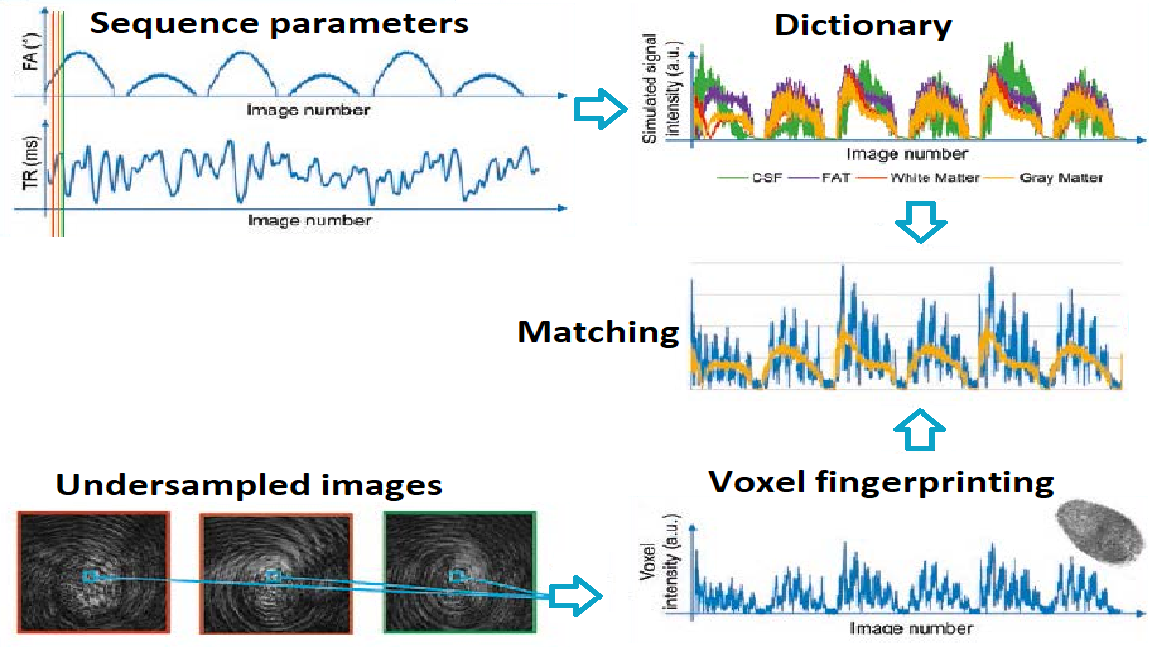
\includegraphics[scale=0.5]{MRF.png}
  \caption{In alto \'e mostrata la generazione del dizionario, mentre in basso si ha la misura effettuata. Viene poi effettuato il matching per determinare quale segnale del dizionario si avvicina a quello effettivamente misurato.}
  \label{MRFpng}
 \end{figure}
 
 
 \chapter{Reti neurali}  
 Il caso pi\'u semplice di rete neurale \'e il percettrone mostrato in figura \ref{perceptronpng}, introdotto da Rosenblatt nel 1958 \cite{rosenblatt1958perceptron}. 
 Con esso, senza ancora introdurre alcuna funzione di attivazione (di cui spiego il ruolo nel capitolo seguente), si possono gi\'a rappresentare tutte le funzioni che sono linearmente separabili come l'AND, l'OR, il NAND o lo XOR. 
 In figura \ref{NeuralNetworkpng} viene mostrata invece la rete neurale, dove il percettrone \'e l'elemento base e ricorsivo della rete. 
 
 L'idea della struttura nasce dalla ricerca di creare un algoritmo che lavori in modo analogo al cervello umano, costituito da unit\'a fondamentali chiamate neuroni, fortemente interconnessi tra loro. 
 La potenza del modello non risiede tanto nell'attivit\'a del singolo neurone, in quanto svolge un calcolo semplice, ma risiede principalmente nella configurazione delle connessioni tra neuroni e nel potere di generalizzazione di questo modello, capace quindi di adattarsi al cambiamento di input senza dover riprogettare i criteri di output.
 
 \begin{figure}[h!]
  \centering
  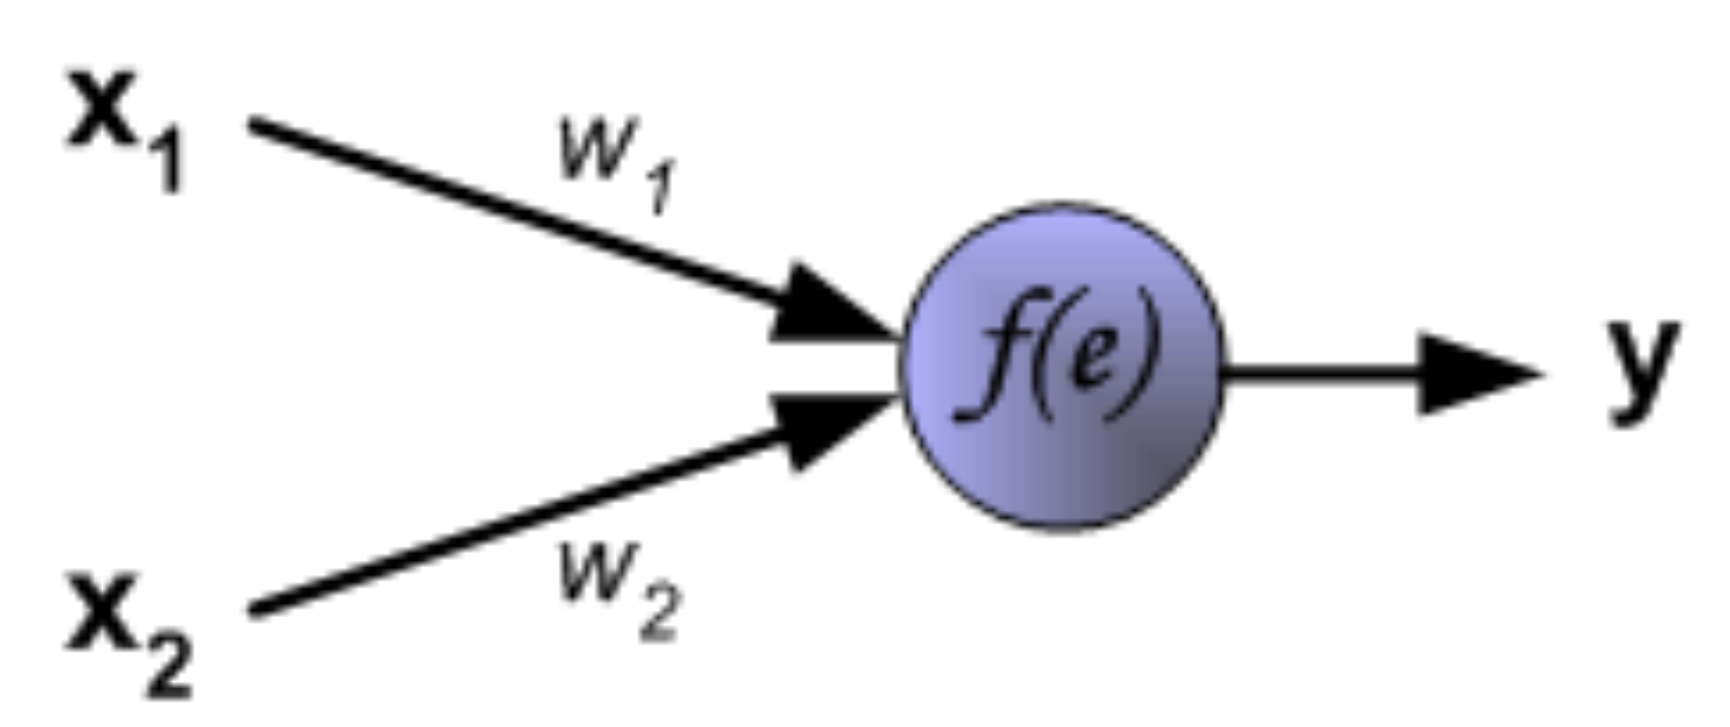
\includegraphics[scale=0.3]{perceptron.png}
  \caption{Percettrone con input composto da due neuroni $x_1$ e $x_2$, un unico neurone nel layer centrale e un output $y$. Il valore del neurone del layer 1 \'e dato da $f(e)$ con $e$ dato dalla somma pesata tra $x_1$ e $x_2$ e i pesi che sono rispettivamente $w_1$ e $w_2$.}
  \label{perceptronpng}
 \end{figure}
 
 \begin{figure}[h!]
  \centering
  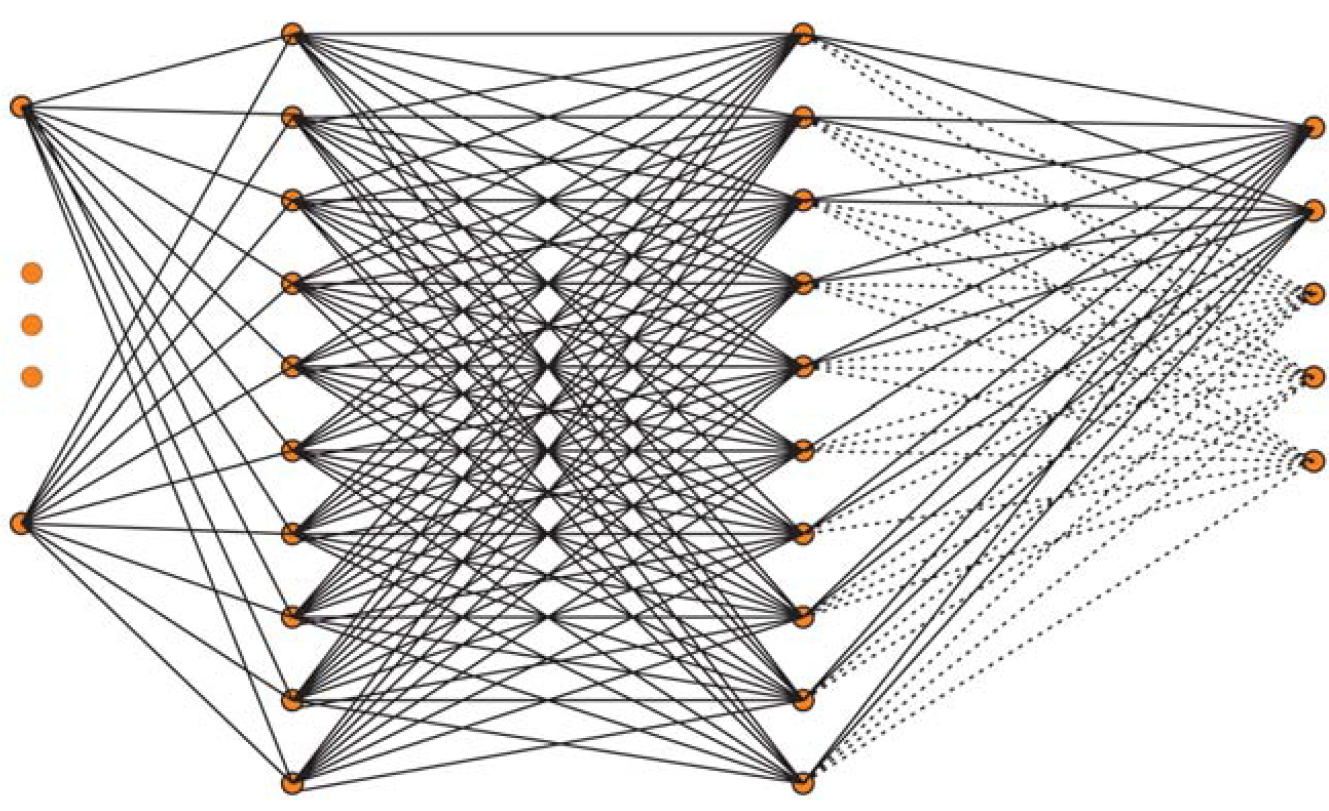
\includegraphics[scale=0.35]{NeuralNetwork.png}
  \caption{Struttura di una rete neurale. Ogni neurone definito dal cerchio arancione si comporta in modo analogo al percettrone visto in precedenza, con la differenza che l' ``output'' viene nuovamente combinato, come se fosse uno dei neuroni di input del layer successivo. L'operazione si ripete per il numero di layer, fino a giungere all'output della rete. Continuando l'analogia con la figura \ref{perceptronpng}, i pesi $w_i$ non sono segnati esplicitamente, ma ne viene associato uno ad ognuno dei collegamenti tra neuroni graficati con le linee nere e cos\'i vale anche per le funzioni d'attivazione associate ai cerchi arancioni: solitamente viene utilizzata la stessa per tutti i neuroni, ma ci sono esempi di lavori in cui si \'e preferito applicare una funzione d'attivazione diversa, per esempio, ai neuroni che costituiscono l'output rispetto a tutti gli altri.}
  \label{NeuralNetworkpng}
 \end{figure}

 \section{Struttura} 
 Partendo dal caso pi\'u semplice mostrato in figura \ref{perceptronpng} si visualizzano gli elementi fondamentali che costituiscono una rete neurale. 
 L'input $x$ \'e composto da un determinato numero di ``neuroni'' ed \'e da essi che il segnale comincia a propagarsi. 
 Ogni unit\'a che costituisce l'input \'e collegato con il neurone del layer centrale, propagando quindi il segnale. 
 Ad ogni collegamento si associa un peso ($w_1$ e $w_2$ in figura \ref{perceptronpng}) che determina l'influenza del ``neurone'' precedente nella propagazione del segnale e una eventuale funzione di attivazione ($f(e)$ in figura \ref{perceptronpng}) viene applicata al segnale finale per introdurre la non linearit\'a nel sistema, definendo quindi il valore finale del percettrone del layer centrale. 
 Nel caso del percettrone tale valore pu\'o essere direttamente l'output a meno di eventuali fattori moltiplicativi, altrimenti, nelle reti come in figura \ref{NeuralNetworkpng} tale processo viene poi ripetuto di layer in layer fino ad arrivare all'output della rete.
  
 Testi diversi suggeriscono funzioni d'attivazione diverse, a seconda del problema affrontato. 
 Attualmente non sembra esistere una funzione d'attivazione che prevalga in modo assoluto per prestazioni, ma la ReLU descritta a breve in equazione \ref{ReLU} pare essere una delle pi\'u utilizzate. 
 Mostro comunque altre tra le funzioni di attivazione pi\'u incontrate:
 \begin{itemize}
  \item Threshold Logic Units, cio\'e funzioni a gradino:
    \begin{equation}
     f(x) = \begin{cases}
             0 & \mbox{se} \;\;\; x<\alpha \\
             1 & \mbox{se} \;\;\; x \ge \alpha
            \end{cases}
    \end{equation}
    con $\alpha$ che si aggiunge ai parametri della rete;

  
  \item Funzioni lineari:
    \begin{equation}
     f(x) = \alpha x + \beta;
    \end{equation}
    con $\alpha$ e $\beta$ che si aggiungono ai parametri della rete;

  
  \item Sigmoidi:
    \begin{equation}
     f(x) = \frac{1}{1+e^{-x}};
    \end{equation}

  
  \item tangenti iperboliche
    \begin{equation}
     f(x) = tanh(x)
    \end{equation}

  
  \item gaussiane
    \begin{equation}
     f(x) = \frac{1}{\sqrt{2 \pi \sigma^2}} e^{-\frac{1}{2}\left(\frac{x-\mu}{\sigma}\right)^2}
    \end{equation}
    con $\sigma$ e $\mu$ che si aggiungono ai parametri della rete;

  
  \item Rectifier Linear Units (ReLU)
    \begin{equation}
     f(x) = ReLU(x) = \mbox{max}(0;x); \label{ReLU}
    \end{equation}

  
  \item Leaky ReLU
    \begin{equation}
     f(x) = LeakyReLU(x) = \begin{cases}
                            \lambda x & \mbox{se} \;\;\; x<0 \\
                            x & \mbox{se} \;\;\; x \ge 0
                           \end{cases}
;\label{LeakyReLU}
    \end{equation}
    con $\lambda$ solitamente <<1 che si aggiunge ai parametri della rete;
    
 \end{itemize}
 
 Passando all'approssimare funzioni pi\'u complesse si introduce la rete neurale in figura \ref{NeuralNetworkpng}, in cui ogni elemento di ogni layer si comporta in modo analogo al percettrone.

 
 \section{Dinamica}
 
 La dinamica di una rete neurale specifica come il segnale si propaghi lungo la rete. 
 Il numero di neuroni del primo layer definisce la dimensione del vettore $x$ dell'input per la determinata rete neurale. 
 Definiamo poi $x_i$ l'$i$-esimo elemento dell'input. 
 Il segnale viene propagato attraverso la somma pesata dei valori dell'input (i pesi sono i parametri principali che la rete dovr\'a apprendere).
 \begin{equation}
  a_j = \sum_{i=1}^n w_i o_i
 \end{equation}
 con $j$ che indica che stiamo considerando il $j$-esimo neurone del layer successivo e $o_i$ (che in questo caso \'e l'input) la componente $i$-esima del segnale che si sta propagando dal layer precedente. 
 Il valore finale del $j$-esimo neurone del nuovo layer \'e dato quindi da $f(a_j)$ con $f$ la funzione di attivazione citata in precedenza. 
 Il segnale $o$ si propaga nella maniera appena descritta un layer dopo l'altro finch\'e i termini $o_k$ non definiscono l'output della rete.
 
 \section{Apprendimento}
 
 La definizione di una rete neurale si completa introducendo quello che \'e l'aspetto principale di questo algoritmo: l'apprendimento. 
 La rete neurale apprende dagli esempi contenuti nel set di training $\tau = \{ z_1, \cdots ,z_n \} $. Il training set differisce a seconda che l'apprendimento sia supervisionato: $\tau = \{ (x_1,\widehat{y}_1), \cdots , (x_n,\widehat{y}_n)\}$ o non supervisionato: $\tau = \{x_1,\cdots,x_n\}$.
 Nel caso di apprendimento supervisionato si ha a disposizione un numero di casi etichettati, di conseguenza, una volta dati in analisi alla rete, si riesce a quantificare l'errore della rete confrontando l'output con l'etichetta a disposizione. 
 In questo caso (che \'e anche quello che viene approfondito di seguito) si riesce ad agire in modo diretto sui parametri della rete. 
 L'apprendimento non supervisionato prevede invece che le informazioni inserite all'interno della rete non siano codificate, dovr\'a essere essa stessa, quindi, a catalogare tutte le informazioni in proprio possesso e organizzarle.
 
 L'apprendimento \'e un processo di modifiche progressive effettuate ai parametri della rete (principalmente i pesi, ma, come visto pocanzi, anche le funzioni di attivazione possono avere parametri da includere nell'apprendimento). 
 Lontano dall'essere un metodo di memorizzazione dei dati del set di training, si suppone che le regole imparate in questo modo riescano a generalizzare il problema, permettendo alla rete di catalogare anche input mai visti in precedenza.
 
 Il processo di modifica dei parametri, nel caso di apprendimento supervisionato, avviene attraverso la back-propagation. Descrivo di seguito come avviene.
 
 Dato l'output $y_i$ della rete, si definisce una funzione di costo, per esempio:
 \begin{equation}
  C(\tau,w) = C(W) = \frac{1}{2} \sum_{i=1}^n (\widehat{y}_i-y_i)^2.
 \end{equation}
 
 Per un peso generico, la correzione applicata durante la back-propagation \'e data da:
 \begin{align}
  w' &= w + \Delta w \\
  \Delta w &= - \eta \frac{\partial C}{\partial w}
 \end{align}
 con $\eta$ tasso di apprendimento da fissare a priori.
 
 Sia $l$ il numero di layer della rete, chiamiamo $L_0$ l'input, $L_l$ l'output e $L_1, \cdots, L_{l-1}$ gli hidden layer. 
 Con $k \in L_j$ indichiamo il $k$-esimo neurone del layer $L_j$.
 L'obiettivo attuale \'e quello di calcolare $\Delta w = - \eta \frac{\partial C}{\partial w}$ per un peso $w$ generico della rete. 
 Consideriamo il peso $w_{ij}$, con $j \in L_{l-1}$ e $i \in L_l$, allora in un hidden layer si ha:
 \begin{align}
  \frac{\partial C}{\partial w_{jk}} &= \frac{\partial}{\partial w_{jk}} \left \{ \frac{1}{2} \sum_{i=1}^m (\widehat{y}_i -y_i)^2 \right \} \\
  &= \frac{\partial}{\partial o_j} \left \{ \frac{1}{2} \sum_{i=1}^m (\widehat{y}_i - y_i)^2 \right \} \frac{\partial o_j}{\partial w_{jk}} \notag \\
  &= \left \{ \frac{1}{2} \sum_{i=1}^m \frac{\partial}{\partial o_j} (\widehat{y}_i - y_i)^2 \right \} \frac{\partial o_j}{\partial w_{jk}} \notag \\
  &= \left \{ - \sum_{i=1}^m (\widehat{y}_i - y_i) \frac{\partial y_i}{\partial o_j} \right \} \frac{\partial o_j}{\partial w_{jk}} \notag \\
  \frac{\partial y_i}{\partial o_j} &= \frac{\partial f_i(a_i)}{\partial a_i} \frac{\partial a_i}{\partial o_j} \\
  &= \dot{f}_i(a_i) \frac{\partial}{\partial o_j} \sum_j w_{ij} o_{ij} \notag \\
  &= \dot{f}_i(a_i) w_{ij} \notag
 \end{align}
 \begin{align}
  \Rightarrow \frac{\partial C}{\partial w_{jk}} &= \left \{ - \sum_{i=1}^m (\widehat{y}_i - y_i) \dot{f}_i(a_i) w_{ij} \right \} \frac{\partial o_j}{\partial w_{jk}} \\
  &= - \left( \sum_{i=1}^m w_{ij} \delta_i \right) \frac{\partial f_j(a_j)}{\partial a_j} \frac{\partial a_j}{\partial w_{jk}} \notag \\
  &= - \left( \sum_{i=1}^m w_{ij} \delta_i \right) \dot{f}_j(a_j) o_k \notag
 \end{align}
 \begin{equation}
  \Rightarrow \Delta w_{jk} = - \eta \frac{\partial C}{\partial w_{jk}} = \eta \left(\sum_{i=1}^m w_{ij} \delta_i \right) \dot{f}_j(a_j) o_k
 \end{equation}
 con $\delta_i = (\widehat{y}_i - y_i) \dot{f}_i(a_i)$.
 
 Definendo:
 \begin{equation}
  \delta_j = \begin{cases}
                       (\widehat{y}_j - y_j) \dot{f}_j(a_j) & \mbox{se} \;\; j \in L_l \\
                       \left( \sum_{i \in L_{k+1}} w_ij \delta_i \right) \dot{f}_j(a_j) & \mbox{se} \;\; j \in L_k \;\; \mbox{dove} \;\; k = l-1,\cdots,0
                      \end{cases}
 \end{equation}
 allora possiamo generalizzare la correzione da applicare ad un peso di un layer qualsiasi come:
 \begin{equation}
  \Delta w_{jk} = \eta \delta_j o_k
 \end{equation}

 \begin{figure}[h!]
  \centering
  \begin{subfigure}[b]{0.45\linewidth}
   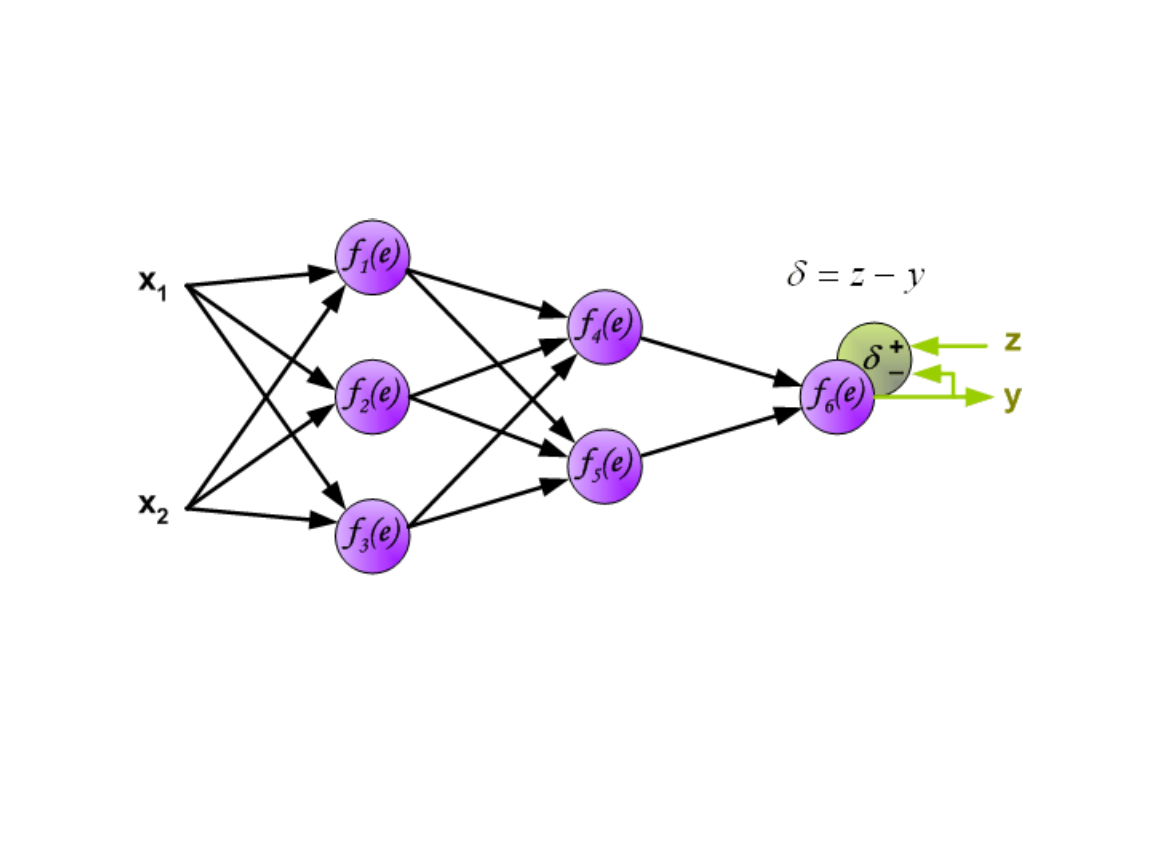
\includegraphics[width=\linewidth]{BackPropa.png}
  \end{subfigure}
  \begin{subfigure}[b]{0.45\linewidth}
   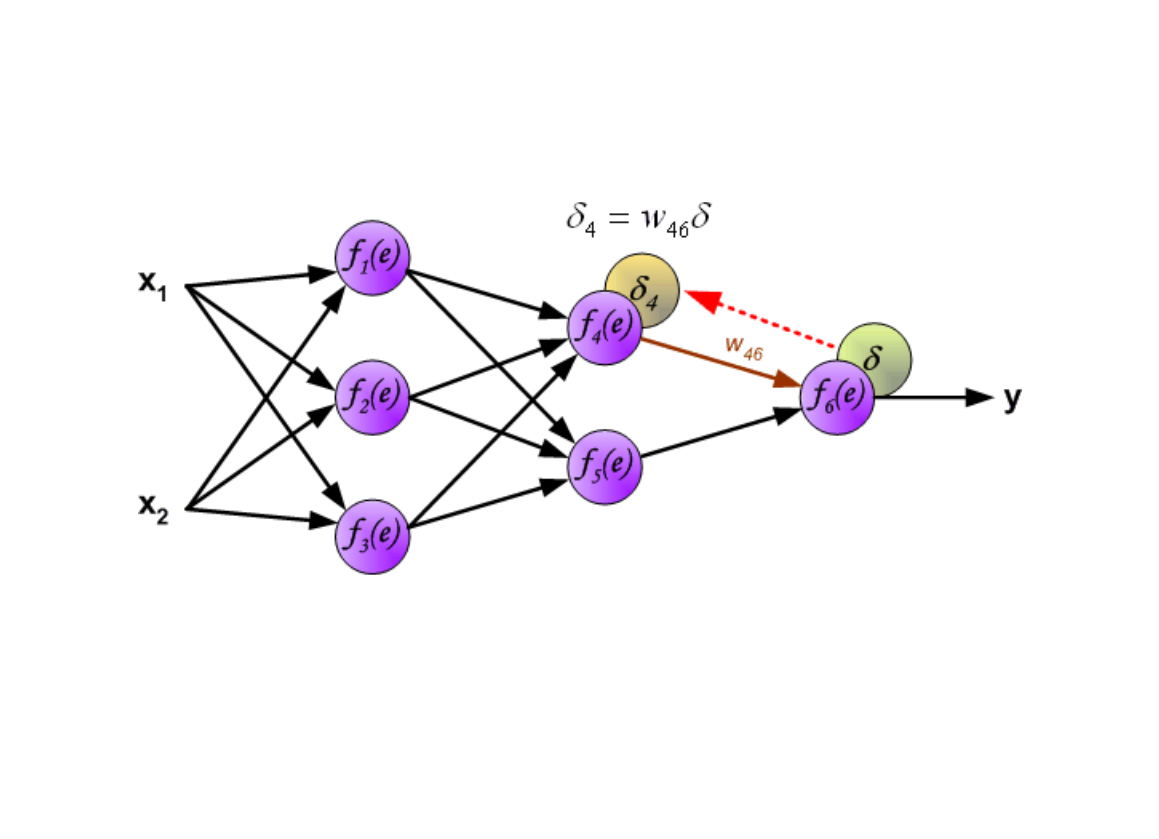
\includegraphics[width=\linewidth]{BackPropb.png}
  \end{subfigure}
  \\
  \begin{subfigure}[b]{0.45\linewidth}
   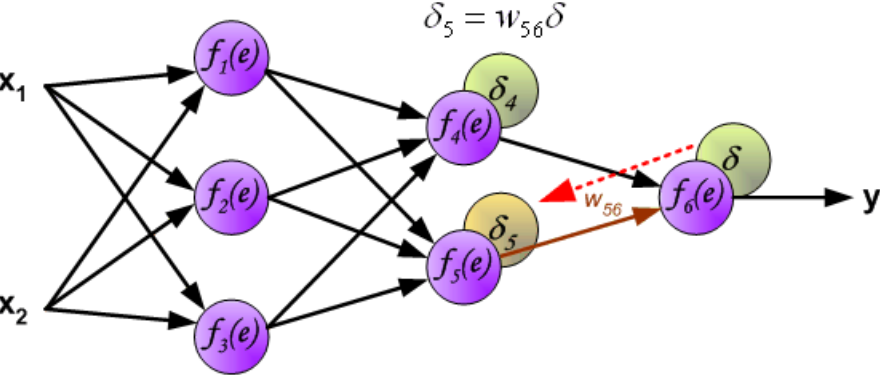
\includegraphics[width=\linewidth]{BackPropc.png}
  \end{subfigure}
  \begin{subfigure}[b]{0.45\linewidth}
   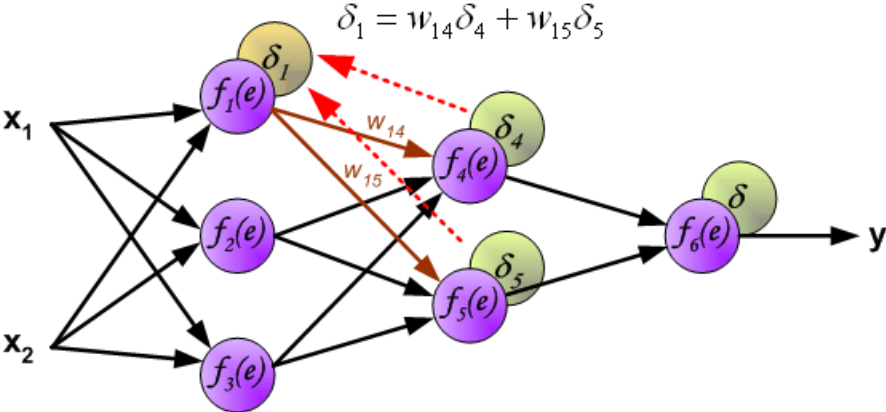
\includegraphics[width=\linewidth]{BackPropd.png}
  \end{subfigure}
  \\
  \begin{subfigure}[b]{0.45\linewidth}
   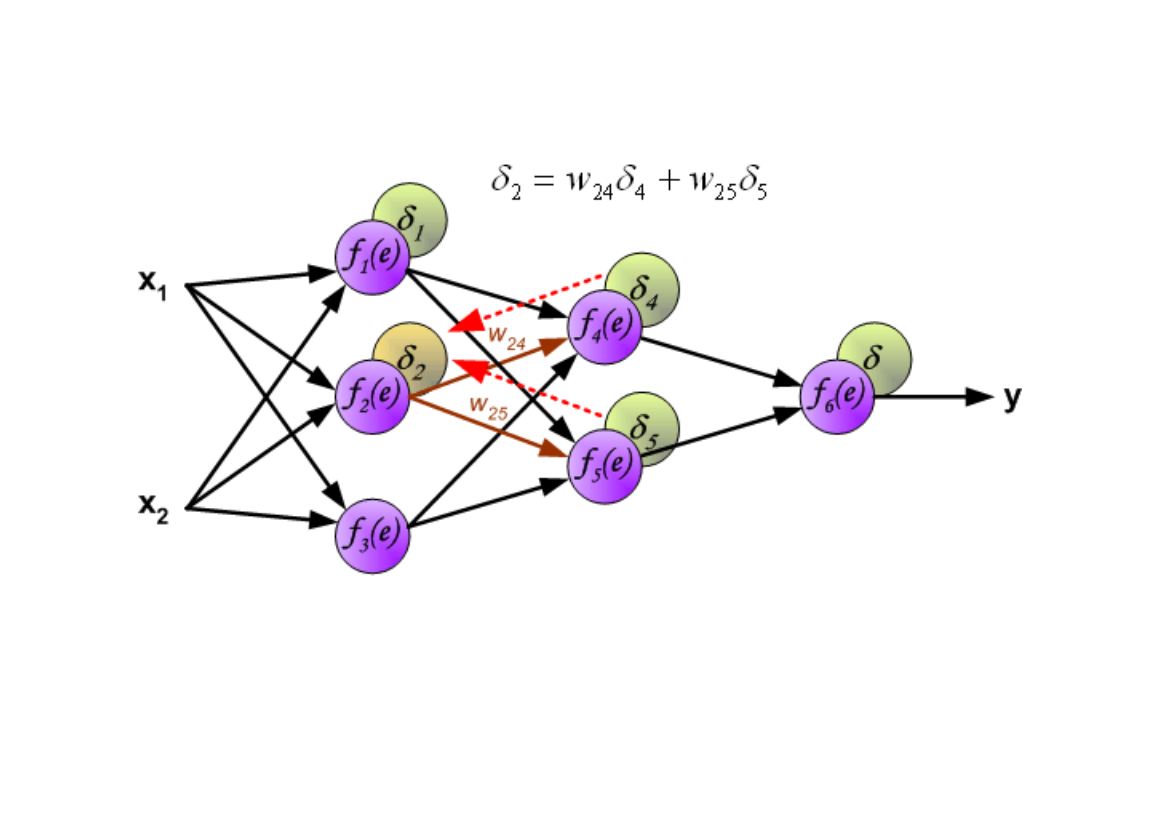
\includegraphics[width=\linewidth]{BackPrope.png}
  \end{subfigure}
  \begin{subfigure}[b]{0.45\linewidth}
   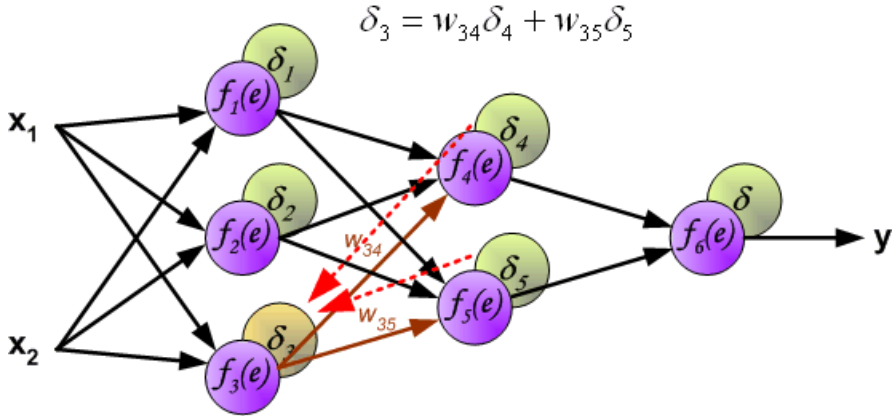
\includegraphics[width=\linewidth]{BackPropf.png}
  \end{subfigure}
  \caption{Utilizzando la nomenclatura introdotta in questo capitolo si visualizzano i valori di $\delta_j$ dovuti alla back propagation, rispettando l'effettivo ordine in cui vengono calcolati.}
 \end{figure}
 Volendo il pi\'u delle volte definire la percentuale di successo della rete e avendo solitamente un set finito $\{(x_1,\widehat{y}_1), \cdots , (x_N,\widehat{y}_N)\}$, si sceglie il set di training con $n<N$ per poter utilizzare gli esempi rimanenti come set di convalida $\zeta = \{(x_{n+1},\widehat{y}_{n+1}), \cdots , (x_N,\widehat{y}_N)\}$. 
 Applicando la rete su questi nuovi input si riesce quindi a stimare l'efficacia della rete neurale.

 
 \chapter*{Reti neurali a valori complessi}
 Le reti neurali a valori complessi sono applicate in sempre pi\'u circostanze. 
 Vengono utilizzate per esempio per rilevare difetti nei metalli analizzando le risposte dei materiali agli ultrasuoni \cite{birx1993complex}, nella ``voice processing'' \cite{sawada2003polar} e nell'analisi dei segnali sonar per la stima di informazioni su un determinato paesaggio \cite{yamaki2008singular}.
 
 
 \section{Storia}
 Uno dei primi esempi di rete neurale fu il percettrone di Rosenbatt (1958) \cite{rosenblatt1958perceptron}. Di seguito fu creata ADELINE (Widrow \& Hoff, 1960) \cite{widrow1962generalization}, composta da un singolo layer con un singolo neurone e utilizzava il $LMS$ (least mean square) insieme ad un algoritmo di discesa stocastica del gradiente per la configurazione dei pesi. 
 Ne descriviamo adesso le caratteristiche. Siano $x \in R^N$ gli input e $w \in R^N$ i pesi; dal modello abbiamo:
 \begin{equation}
  y = x \cdot w.
 \end{equation}
 Dato l'output desiderato $\widehat{y} \in R$ possiamo definire la funzione errore $e$ e la $loss \ function \ L$. 
 L'obiettivo \'e quello di trovare il valore dei pesi che minimizzi $L$.
 \begin{align}
  e &= \widehat{y} - y\\
  L &= e^2\\
  w &\leftarrow arg \, min(L).
 \end{align}
 L'algoritmo $LMS$ ottimizza $L$ usando il gradiente discendente:
 \begin{align}
  \nabla L_w: &= -2ex\\
  w &\leftarrow w + \eta ex
 \end{align}
 dove $\eta$ \'e il tasso di apprendimento. 

 Widrow, McCool and Ball (1975) \cite{widrow1975complex} hanno esteso l'algoritmo $LMS$ al dominio complesso fornendo la derivazione delle parti reali e immaginarie. 
 Brandwood (1983) \cite{brandwood1983complex} generalizz\'o la teoria applicando il gradiente al numero complesso, senza separarlo in parte reale e parte immaginaria attraverso il gradiente di Wirtinger (1927) \cite{wirtinger1927formalen}. 

 Aggiorniamo quindi il problema nel dominio complesso:
 \begin{align}
  L &= e \overline{e}\\
  \nabla L_w : &= -2e\overline{x}\\
  w &\leftarrow w + \eta e \overline{x}.
 \end{align}
 Nonostante i risultati di Brandwood, fino a non molto tempo fa la letteratura non applicava il calcolo di Wirtinger, a favore della derivazione separata della parte reale da quella immaginaria. 
 
 \section{Struttura}
 Esaminiamo un modello $feedforward$ avente un unico hidden layer; abbiamo di conseguenza:
 \begin{align}
  h &= f\left(W^{\left(h\right)}x+b^{\left(h\right)}\right)\\
  y &= W^{\left(o\right)}x+b^{\left(o\right)}
 \end{align}
 con $\theta = \left \{ W^{\left(h\right)}, \ W^{\left(o\right)}, \ b^{\left(h\right)}, \ b^{\left(o\right)}\right \}$ sono i parametri del modello. Definendo $M$ il numero dei nodi dell'input e $N$ il numero dei nodi dell'output, avremo:
 \begin{equation}
  \begin{matrix}
   W^{\left( h\right) } \in R^{M\times M} & or & W^{\left( o\right) } \in C^{M\times M}\\
   b^{\left( h\right) } \in R^M & or & b^{\left( o\right) } \in C^M\\
   W^{\left( o\right) } \in R^{N\times M} & or & W^{\left( o\right) } \in C^{N\times M}\\
   b^{\left( o\right) } \in R^N & or & b^{\left( o\right) } \in C^N
  \end{matrix}
 \end{equation}
 In tutti i casi gli input, i pesi e gli output appartengono allo stesso dominio numerico.
 
 \section{Funzione d'attivazione}
 
 Bisogna ricordare che la funzione d'attivazione deve essere una funzione $f(x):C \to C$ e un aspetto fondamentale che interessa la back-propagation \'e la derivabilit\'a. 
 Tenendo conto di ci\'o, riporto di seguito le funzioni d'attivazione che ho trovato essere quelle pi\'u utilizzate per reti neurali a valori complessi.
 \begin{description}
 \item[Identit\'a]
 Permette una modellizazione lineare
 \begin{equation}
  f^{\left(-\right) }\left(x\right) := x
 \end{equation}

 \item[Tangente Iperbolica]
 \'E una funzione sigmoidale e differenziabile. Permette una non linearit\'a ampiamente utilizzata per l'apprendimento delle reti neurali
 \begin{equation}
  f^{\left(\sigma\right) } := tanh\left( x\right)
 \end{equation}

 \item[Split reale-immaginario]
 Applica la tangente iperbolica separatamente alla parte reale e alla parte immaginaria:
 \begin{equation}
  f^{\left( ri\right)} \left( x\right) := tanh\left( Re \ x\right) +i \ tanh\left( Im \ x\right)
 \end{equation}

 \item[Split ampiezza-fase]
 Applica la tangente iperbolica al modulo del numero complesso, senza modificarne la fase (questa funzione non \'e differenziabile nel campo complesso)
 \begin{equation}
  f^{\left( ap\right) } \left( x\right) := tanh\left( \left| x\right|\right) e^{i \, arg \, x}
 \end{equation}
 
 \item[ModReLU]
 Arjosky nel 2015 propose una variazione alla classica ReLU utilizzata nelle reti neurali reali, definita come segue:
 \begin{equation}
  ModReLU\left( z\right) = ReLU\left( \left| z\right|+b\right) e^{i\theta_z} = \begin{cases}
                                                                                               \left(\left| z\right| +b\right) \frac{z}{\left| z\right|} & \mbox{se} \left| z\right| +b \ge 0 \\
                                                                                0 & \mbox{altrimenti}
                                                                
                                                                \end{cases}
 \end{equation}
 dove $\theta_z$ \'e la fase di $z$ e $b$ il bias, apprendibile dalla rete neurale, e necessario per creare una $dead \ zone$ di raggio b attorno all'origine dove il neurone \'e inattivo. Tale funzione non soddisfa le equazioni di Cauchy-Riemann e quindi non \'e olomorfa.
 
 \item[CReLU]
 Consiste in una applicazione della funzione ReLu individualmente alla parte reale e alla parte immaginaria:
 \begin{equation}
  CReLU\left( z\right) = ReLU\left( Re\left( z\right)\right) + i \, ReLU\left( Im\left( z\right)\right).
 \end{equation}
 Questa soddisfa le condizioni di Cauchy-Riemann solo se sia la parte reale che la parte immaginaria sono contemporaneamente strettamente positive o strettamente negative, quindi nell'intervallo $\theta_z \in \left( 0, \frac{\pi}{2}\right)$ oppure $\theta_z \in \left( \pi, \frac{ 3 \pi}{2}\right)$.
 
 \item[zReLU]
 Proposta nel 2016 da Guberman e basata anch'essa sulla ReLu, \'e definita come:
 \begin{equation}
   zReLU\left( z\right) = \begin{cases}
                                                                                               z & \mbox{se} \theta_z \in \left[ 0, \frac{ \pi}{2}\right] \\
                                                                                0 & \mbox{altrimenti}
                                                             
                                                     \end{cases}
 \end{equation}

\end{description}
 
 \section{Back propagation}
 
 \subsection{Loss function}
 La maggior parte della letteratura attuale utilizza come funzione di costo la $mean$ $squarred$ $error$. 
 Dato un target $\widehat{y}$ e l'output ottenuto $y$, entrambi in $C^N$ e l'errore: 
 \begin{equation}
  e:=\widehat{y}-y \label{error}
 \end{equation}
 la $complex$ $mean$ $squared$ $loss$ $function$ \'e definita come segue:
 \begin{align}
  L(e) &= \sum_{i=0}^{N-1} \left| e_i\right|^2\label{lossF}\\
  &=\sum_{i=0}^{N-1} e_i \overline{e_i}. \notag
 \end{align}
 La \ref{lossF} \'e una funzione a valori reali scalari non negativi, che tende a zero insieme al modulo dell'errore. 
 Savitha, Suresh e Sundararajan \cite{savitha2009new} proposero di sostituire l'errore \ref{error} con:
 \begin{equation}
  e:=log ( \widehat{y} ) - log ( y ).\label{complexError}
 \end{equation}
 La $loss$ $function$ diventerebbe quindi:
 \begin{equation}
  L(e)=\left( log\left| \widehat{y_i}\right|-log\left| y_i\right|\right)^2 + \left(arg( \widehat{y_i}) - arg  (y_i)\right)^2 \label{complexLossF}
 \end{equation}
 L'equazione \ref{complexLossF} ha la propriet\'a di rappresentare esplicitamente l'ampiezza e la fase.
 Le equazioni \ref{error} e \ref{complexError} possono essere $error$ $function$ appropriate per reti neurali complesse.
 
 \subsection{Il gradiente complesso ed il calcolo di Wirtinger}
 Wirtinger (1927) \cite{wirtinger1927formalen} forn\'i un formalismo che rese il calcolo della derivata di funzioni con valori complessi meno oneroso rispetto a funzioni olomorfe e non analitiche, agendo interamente nel campo complesso. 
 Nonostante tale apparente comodit\'a, solo recentemente si ricominci\'o ad utilizzare il calcolo di Wirtinger per la $back-propagation$ di reti neurali complesse. 

 Definiamo:
 \begin{align}
  f(z) : &= f\left( z,\overline{z}\right)\\
  &= g\left( x,y\right) \notag \\
  &= u\left( x,y\right) +iv\left( x,y\right) \notag
 \end{align}
 con $z\in C$, $x,y\in R$ e $z=x+iy$. 

 Usando la prima definizione avremo le derivate in $z$ e $\overline{z}$ date da:
 \begin{align}
  \frac{\partial f}{\partial z}\bigg|_{\overline{z} \ costante}\\
  \frac{\partial f}{\partial \overline{z}}\bigg|_{z \ costante}
 \end{align}
 le quali, espresse in funzioe di $x$ e $y$, diventano:
 \begin{align}
  \frac{\partial f}{\partial z} = \frac{1}{2}\left(\frac{\partial f}{\partial x}-i\frac{\partial f}{\partial y}\right)\label{derivatafz}\\
  \frac{\partial f}{\partial \overline{z}} = \frac{1}{2}\left(\frac{\partial f}{\partial x}+i\frac{\partial f}{\partial y}\right).\label{derivatafzcon}
 \end{align}
 Si osservi che la derivata parziale rispetto a $\overline{z}$ \'e nulla per ogni funzione olomorfa. 
 Richiamiamo le condizioni di esistenza di Cauchy-Riemann per la derivata complessa della funzione $f(z,\overline{z})$ presa in considerazione:
 \begin{align}
  \frac{\partial u}{\partial x} &= \frac{\partial v}{\partial y}\\
  \frac{\partial v}{\partial x} &=- \frac{\partial u}{\partial y}.
 \end{align}
 Se applichiamo le condizioni di Cauchy-Riemann alla derivata di $f$ in $\overline{z}$ \ref{derivatafzcon} notiamo che effettivamente essa si annulla. 
 Le funzioni olomorfe quindi non dipendono esplicitamente da $\overline{z}$. 
 Brandwood dimostr\'o che l'annullarsi di \ref{derivatafz} o \ref{derivatafzcon} per una generica $f:C\rightarrow R$ \'e condizione sufficiente e necessaria affinch\'e $f$ abbia un punto stazionario. 
 Per estensione se $f:C^N\rightarrow R$ \'e una funzione a valori reali di un certo vettore $z=\left[ z_0, \ z_1, \ \cdots \ , \ z_{N-1}\right]^T \in C^N$ e definiamo il cogradiente e il gradiente coniugato come:
 \begin{align}
  \frac{\partial}{\partial z} &:=\left[ \frac{\partial}{\partial z_0},\frac{\partial}{\partial z_1},\cdots ,\frac{\partial}{\partial z_{N-1}}\right]\\
  \frac{\partial}{\partial \overline{z}} &:=\left[ \frac{\partial}{\partial \overline{z_0}},\frac{\partial}{\partial \overline{z_1}},\cdots ,\frac{\partial}{\partial \overline{z_{N-1}}}\right]
 \end{align}
 allora $\frac{\partial f}{\partial z}=0$ o $\frac{\partial f}{\partial \overline{z}}=0$ sono condizioni sufficienti e necessarie per determinare un punto di stazionariet\'a. 

 Se $f$ \'e una funzione di un vettore complesso $z$, la sua derivata totale \'e:
 \begin{equation}
  df=\frac{\partial f}{\partial z}dz+\frac{\partial f}{\partial \overline{z}}d\overline{z}.
 \end{equation}
 Se $f$ \'e reale allora avremmo:
 \begin{equation}
  df=2Re\left \{ \frac{\partial f}{\partial z} dz \right \}.
 \end{equation}
 Definendo ora l'operatore gradiente come:
 \begin{align}
  \nabla_z :&= \left(\frac{\partial}{\partial\overline{z}}\right)^T\\
  &=\left(\frac{\partial}{\partial z}\right)^* \notag
 \end{align}
 pu\'o essere dimostrato, usando la disuguaglianza di Cauchy-Scharz, che $f$ ha il maggior tasso di cambiamento lungo il gradiente. Grazie a queste definizioni possiamo costruire una $cost \, function$ reale con argomenti complessi anche se alcuni elementi della funzione non sono olomorfi. 
 In generale, date le funzioni arbitrarie $f$e $g$, combiniamo gli jacobiani come segue
 \begin{align}
  J_{f\circ g} = J_f J_g + J_f^{\left(c\right)}\overline{\left(J_g^{\left(c\right)}\right)}\\
  J_{f\circ g}^{\left(c\right)} = J_f J_g^{\left(c\right)} + J_f^{\left(c\right)}\overline{\left(J_g\right)}.
 \end{align}
 Supponiamo di avere una funzione composta $\left(f\circ g\circ h\right)\left(z,\overline{z}\right)$, con $f$ la $cost \, function$ reale, $g$ una funzione complessa non olomorfa e $h$ una funzione olomorfa. 
 Tenendo a mente che $f$ \'e una funzione a valori reali di variabile complessa e che $h$ \'e olomorfa ( $\frac{\partial h}{\partial \overline{z} = 0}$ ), applichiamo la $chain \ rule$:
 \begin{align}
  J_f &= \frac{ \partial f}{ \partial g}\\
  J_f^{\left( c\right)} &= \frac{\partial f}{\partial \overline{g}}\\
  J_{f\circ g} &= J_f \frac{\partial g}{\partial h} + J_f^{\left( c\right)} \overline{\left( \frac{\partial g}{\partial \overline{h}}\right) }\\
  J_{f\circ g\circ h} &= J_{f\circ g} \frac{\partial h}{\partial z}\\
  \nabla_z f &= \left( J_{f\circ g\circ h}\right)^*
 \end{align}
 Il Calcolo di Wirtinger rende un po' pi\'u semplice costruire un grafico computazionale per reti complesse aventi composizioni miste di operazioni olomorfe e non olomorfe.
 
 \section{Confronto con rete neurale a valori reali} \label{CompR-Csection}
 
 Le reti neurali a valori complessi non sono un nuovo concetto, tuttavia, l'uso di modelli a valore reale \'e stato spesso favorito rispetto a modelli a valore complesso a causa delle difficolt\'a nella formazione e nelle prestazioni, infatti, come riprender\'o pi\'u avanti, le reti neurali complesse non sempre convengono e se comparate alle reti neurali a valori reali, soprattutto in problemi naturamente nel dominio reale e non complesso. 
 In tal caso infatti introducendo i numeri complessi si ottengono risultati non molto distanti, ma con una complessit\'a di calcolo maggiore. 
 
 Il numero di parametri reali \'e una metrica per quantificare la capacit\'a di una rete nella sua capacit\'a di approssimare funzioni strutturalmente complesse. 
 Con troppi parametri il modello tende a overfittare i dati mentre con troppi pochi tende a underfittare. Spesso la letteratura per\'o ignora il numero di parametri, finendo col confrontare reti di dimensioni notevolmente diverse.  Bisogna garantire che queste architetture siano comparabili per dimensioni e capacit\'a del modello. 
 Per definire la dimensione della rete si pu\'o considerare il numero di parametri reali. Di conseguenza, per costruire reti comparabili o si imposta un numero fisso di neuroni a valore reale oppure si fissa il numero di parametri reali per ogni rete.
 
 Una conseguenza della rappresentazione di un numero complesso come $a+\textbf{i}b$ (utilizzando quindi due numeri reali) \'e dato dal fatto che, a parit\'a di ``neuroni'', il numero di parametri $p_C$ della rete complessa diventa il doppio del numero di parametri $p_R$ di una rete a valori reali. 
 Per garantire che  modelli abbiano le stesse capacit\'a il numero di parametri a valore reale per layer deve essere uguale o almeno il pi\'u simile possibile. 
 In questo modo le differenze di prestazione sono causate dall'introduzione di numeri complessi come parametri e non da una differenza di capacit\'a. 
 
 Si consideri il numero di parametri in uno strato fully connected nel caso reale e nel caso complesso. 
 Sia $d$ la dimensione dell'input e $m$ il numero di neuroni di un layer, di conseguenza il numero di parametri nel caso reale e nell caso complesso \'e:
 \begin{equation}
  p_R = (d \times m) + m, \;\;\;\; p_C = 2(d \times m) + 2m
 \end{equation}
 Per una rete neurale con $k$ hidden layers e output di dimensione $c$, il numero di parametri reali (senza contare i bias) diventa:
 \begin{align}
  p_R &= d \times m + k(m \times m) + m \times c, \\
  p_C &= 2\left[ d \times m + k(m \times m) + m \times c \right]
 \end{align}
 
 A prima vista la progettazione di architetture di reti neurali multistrato comparabili, ovvero con lo stesso numero di paramentri a valore reale in ogni layer pare banale. 
 Tuttavia, dimezzare il numero di neuroni in ogni stato non permette il raggiungimento della comparabilit\'a dei parametri. 
 Si pu\' affrontare questo problema scegliendo delle architetture con un numero di hiddel layers $k$ e un numero di neuroni per layer che pu\'o alternarsi tra $m$ e $m/2$. 
 
 Si consideri per esempio le dimensioni degli ouput e dei pesi con $k=4$. Per il caso reale si ha quindi:
 
\begin{align}
  (1 \times d)\overbrace{(d \times m_1)}^{Input \; layer} &\to (1 \times m_1)\overbrace{(m_1 \times m_2)}^{Hidden \; layer} \\
  \to (1 \times m_2)\overbrace{(m_2 \times m_3)}^{Hidden \; layer} &\to (1 \times m_3)\overbrace{(m_3 \times m_4)}^{Hidden \; layer} \notag \\
  \to (1 \times m_4)\overbrace{(m_4 \times m_5)}^{Hidden \; layer} &\to (1 \times m_5)\overbrace{(m_5 \times c)}^{Hidden \; layer} \notag \\
  &\to \overbrace{(1 \times c)}^{Model \; ouput} \notag
 \end{align}
Mentre per il caso complesso:
 \begin{align}
  (1 \times n)(n \times m_1/2) &\to (1 \times m_1/2)(m_1/2 \times m_2)\\
  \to (1 \times m_2)(m_2 \times m_3/2) &\to (1 \times m_3/2)(m_3/2 \times m_4) \notag \\
  \to (1 \times m_4)(m_4 \times m_5/2) &\to (1 \times m_5/2)(m_5/2 \times c) \notag \\
  &\to (1 \times c) \notag
 \end{align}
 
 Un ulteriore approccio \'e quello di lavorare pi\'u in generale con un budget di parametri. 
 Quindi dato un numero massimo di parametri reali $p_R$, si definisce una rete neurale a valori reali o complessi con un numero di hidden layer $k \ge 0$ tale da rimanere nel budget. 
 I $k$ hidden layer hanno lo stesso numero di neuroni, reali o complessi che siano : $m_R = m_C$. Il numero di neuroni nell'ultimo layer \'e definito dal numero di classi $c$.
 \begin{align}
  m_R &= \begin{cases}
          -\frac{n+c}{2k} + \sqrt{ \frac{n+c}{2k}^2 + \frac{p_R}{k}}, & \mbox{se} \; k>0\\
          \frac{p_R}{n+c} & \mbox{altrimenti}
         \end{cases} \label{LastLayerR}\\
  m_C &= \begin{cases}
          -\frac{n+c}{2k} + \sqrt{ \frac{n+c}{2k}^2 + \frac{p_R}{k}}, & \mbox{se} \; k>0\\
          \frac{2(p_R)}{n+c} & \mbox{altrimenti}
         \end{cases} \label{LastLayerC}
 \end{align}

 
 Confrontando reti neurali reali e complesse di capacit\'a simile, i modelli complessi hanno prestazioni solitamente uguali o leggermente peggiori rispetto ai modelli a valore reale, se vengono considerati compiti di classificazione nel dominio reale. 
 Tuttavia le reti neurali a valore complesso sono state applicate con successo a una variet\'a di compiti, in particolare nell'elaborazione dal segnale in cui i dati di input hanno una interpretazione fisica nel dominio complesso\cite{birx1993complex} \cite{sawada2003polar} \cite{yamaki2008singular} \cite{hirose2009complex} \cite{guberman2016complex} \cite{trabelsi2017deep}. Il pregio principale delle 
 reti neurali a valore complesso \'e quello di riuscire a gestire meglio il rumore sul piano complesso.
 
 Per confrontare reti neurali a valori reali con quelli a valori complessi, Nils M\"onning e Suresh Manandhar in $Evaluation$ $of$ $Complex-Valued$ $on$ $Real-Valued$ $Classification$ $Tasks$  \cite{monning2018evaluation} applicano entrambe le reti a problemi di classificazione comuni. 
 Gli esperimenti eseguiti sono due:
 \begin{itemize}
  \item MLP con numero di hidden layers $k = 0, 2, 4, 8$, dimensione degli hidden layer fissa per le reti a valori reali e alternante (64 o 32 neuroni) per le reti a valori complessi. Non \'e stato definito un budget di parametri. Il test \'e stato fatto sul problema di classificazione MINST, CIFAR-10, CIFAR-100 e Reuters. 
  \item MLP con budget fisso di 500000 parametri reali. Le dimensioni sono quindi variabili e saranno indicate di volta in volta. Vengono scelti gli stessi problemi di classificazione citati per il caso precedente. Il numero di neuroni dell'ultimo layer \'e definito dalle equazioni \ref{LastLayerR} e \ref{LastLayerC} e viene arrotondato per eccesso.
 \end{itemize}
 
 \'E stata utilizzata l'inizializzazione dei pesi discussa da Trabelsi et al. \cite{trabelsi2017deep} per tutti gli esperimenti. 
 Per ridurre l'impatto dell'inizializzazione, ogni modello \'e stato addestrato 10 volte, con training composte da 100 epochs. 
 Come funzione d'attivazione per l'ultimo layer \'e stata usata sempre la $sigmoid(|z|^2)$ o la $softmax(|z|^2)$.
  
 Le tabelle \ref{MNIST1Tab},\ref{Reuters1Tab},\ref{CIFAR-101Tab},\ref{CIFAR-1001Tab} mostrano i risultati per reti neurali con dimensione variabile e budget illimitato per i parametri (esperimento 1). 
 Le tabelle \ref{MNIST2Tab},\ref{Reuters2Tab},\ref{CIFAR-102Tab},\ref{CIFAR-1002Tab} mostrano invece i risultati dell'esperimento 2.
 
 
 \begin{table}[h]
  \centering
  \begin{tabular}{cp{0.2\textwidth} cp{0.2\textwidth}   cp{0.2\textwidth} cp{0.2\textwidth} cp{0.2\textwidth}}
   \cline{1-5}
   Hidden layers $k$ & Real parameters $p_R$ & Activation function $\phi$ & \multicolumn{2}{c}{MNIST}\\
   \cline{4-5}
   & & & R & C \\
   \cline{1-5}
   & & $identity$ & 0.9282 & 0.9509 \\
   \cline{3-5}
   & & $tanh$ & 0.9761 & 0.9551 \\
   \cline{3-5}
   k=0 & 50816 & $ReLU$ & 0.9780 & 0.9710 \\
   \cline{3-5}
   & & $|z|^2$ & 0.9789 & 0.9609 \\
   \cline{3-5}
   & & $|z|$ & 0.9770 & 0.9746 \\
   \cline{1-5}
  
   & & $identity$ & 0.9274 & 0.9482 \\
   \cline{3-5}
   & & $tanh$ & 0.9795 & 0.8923 \\
   \cline{3-5}
   k=2 & 59008 & $ReLU$ & 0.9804 & 0.9742 \\
   \cline{3-5}
   & & $|z|^2$ & 0.9713 & 0.6573 \\
   \cline{3-5}
   & & $|z|$ & 0.9804 & 0.9755 \\
   \cline{1-5}
  
   & & $identity$ & 0.9509 & 0.9468 \\
   \cline{3-5}
   & & $tanh$ & 0.9802 & 0.2112 \\
   \cline{3-5}
   k=4 & 67200 & $ReLU$ & 0.9816 & 0.9768 \\
   \cline{3-5}
   & & $|z|^2$ & 0.8600 & 0.2572 \\
   \cline{3-5}
   & & $|z|$ & 0.9789 & 0.9738 \\
   \cline{1-5}
   
   & & $identity$ & 0.9242 & 0.1771 \\
   \cline{3-5}
   & & $tanh$ & 0.9796 & 0.1596 \\
   \cline{3-5}
   k=8 & 83584 & $ReLU$ & 0.9798 & 0.9760 \\
   \cline{3-5}
   & & $|z|^2$ & 0.0980 & 0.0980 \\
   \cline{3-5}
   & & $|z|$ & 0.9794 & 0.1032 \\
   \cline{1-5}
  \end{tabular}
  \caption{Tratto da \cite{monning2018evaluation}. Test di accuratezza di reti con $k+2$ layer, ognuno con 64 neuroni (alternando 32 e 64 neuroni nei layer della rete a valori complessi) e un output con $c=10$ neuroni. Esperimento 1.}
  \label{MNIST1Tab}
 \end{table}
 
 \newpage
 
 \begin{table}[h]
  \centering
  \begin{tabular}{cp{0.2\textwidth} cp{0.2\textwidth}   cp{0.2\textwidth} cp{0.2\textwidth} cp{0.2\textwidth}}
   \cline{1-5}
   Hidden layers $k$ & Real parameters $p_R$ & Activation function $\phi$ & \multicolumn{2}{c}{Reuters}\\
   \cline{4-5}
   & & & R & C \\
   \cline{1-5}
   & & $identity$ & 0.8116 & 0.7936 \\
   \cline{3-5}
   & & $tanh$ & 0.8117 & 0.7912 \\
   \cline{3-5}
   k=0 & 642944 & $ReLU$ & 0.8081 & 0.7934 \\
   \cline{3-5}
   & & $|z|^2$ & 0.8050 & 0.7885 \\
   \cline{3-5}
   & & $|z|$ & 0.8068 & 0.7992 \\
   \cline{1-5}
  
   & & $identity$ & 0.8005 & 0.7836 \\
   \cline{3-5}
   & & $tanh$ & 0.7978 & 0.7320 \\
   \cline{3-5}
   k=2 & 651136 & $ReLU$ & 0.7921 & 0.7854 \\
   \cline{3-5}
   & & $|z|^2$ & 0.7725 & 0.6874 \\
   \cline{3-5}
   & & $|z|$ & 0.7996 & 0.7823 \\
   \cline{1-5}
  
   & & $identity$ & 0.7925 & 0.7787 \\
   \cline{3-5}
   & & $tanh$ & 0.7814 & 0.4199 \\
   \cline{3-5}
   k=4 & 659328 & $ReLU$ & 0.7734 & 0.7671 \\
   \cline{3-5}
   & & $|z|^2$ & 0.5895 & 0.0650 \\
   \cline{3-5}
   & & $|z|$ & 0.7863 & 0.7694 \\
   \cline{1-5}
   
   & & $identity$ & 0.7929 & 0.7796 \\
   \cline{3-5}
   & & $tanh$ & 0.7542 & 0.1861 \\
   \cline{3-5}
   k=8 & 675712 & $ReLU$ & 0.7555 & 0.7676 \\
   \cline{3-5}
   & & $|z|^2$ & 0.0053 & 0.0053 \\
   \cline{3-5}
   & & $|z|$ & 0.7671 & 0.7524 \\
   \cline{1-5}
  \end{tabular}
  \caption{Tratto da \cite{monning2018evaluation}. Test di accuratezza di reti con $k+2$ layer, ognuno con 64 neuroni (alternando 32 e 64 neuroni nei layer della rete a valori complessi) e un output con $c=46$ neuroni. Esperimento 1.}
  \label{Reuters1Tab}
 \end{table}
 
 \newpage
 
 \begin{table}[h]
  \centering
  \begin{tabular}{cp{0.2\textwidth} cp{0.2\textwidth}   cp{0.2\textwidth} cp{0.2\textwidth} cp{0.2\textwidth}}
   \cline{1-5}
   Hidden layers $k$ & Real parameters $p_R$ & Activation function $\phi$ & \multicolumn{2}{c}{MNIST}\\
   \cline{4-5}
   & & & R & C \\
   \cline{1-5}
   & & $identity$ & 0.4044 & 0.1063 \\
   \cline{3-5}
   & & $tanh$ & 0.4885 & 0.1431 \\
   \cline{3-5}
   k=0 & 394496 & $ReLU$ & 0.4902 & 0.4408 \\
   \cline{3-5}
   & & $|z|^2$ & 0.5206 & 0.1000 \\
   \cline{3-5}
   & & $|z|$ & 0.5256 & 0.1720 \\
   \cline{1-5}
  
   & & $identity$ & 0.4039 & 0.1000 \\
   \cline{3-5}
   & & $tanh$ & 0.5049 & 0.1672 \\
   \cline{3-5}
   k=2 & 427264 & $ReLU$ & 0.5188 & 0.4960 \\
   \cline{3-5}
   & & $|z|^2$ & 0.1451 & 0.1361 \\
   \cline{3-5}
   & & $|z|$ & 0.5294 & 0.1000 \\
   \cline{1-5}
  
   & & $identity$ & 0.4049 & 0.1000 \\
   \cline{3-5}
   & & $tanh$ & 0.4983 & 0.1549 \\
   \cline{3-5}
   k=4 & 460032 & $ReLU$ & 0.8445 & 0.6810 \\
   \cline{3-5}
   & & $|z|^2$ & 0.1000 & 0.1000 \\
   \cline{3-5}
   & & $|z|$ & 0.5273 & 0.1000 \\
   \cline{1-5}
   
   & & $identity$ & 0.4005 & 0.1027 \\
   \cline{3-5}
   & & $tanh$ & 0.4943 & 0.1365 \\
   \cline{3-5}
   k=8 & 525568 & $ReLU$ & 0.5072 & 0.4939 \\
   \cline{3-5}
   & & $|z|^2$ & 0.1000 & 0.1000 \\
   \cline{3-5}
   & & $|z|$ & 0.5276 & 0.1000 \\
   \cline{1-5}
  \end{tabular}
  \caption{Tratto da \cite{monning2018evaluation}. Test di accuratezza di reti con $k+2$ layer, ognuno con 128 neuroni (alternando 128 e 64 neuroni nei layer della rete a valori complessi) e un output con $c=10$ neuroni. Esperimento 1.}
  \label{CIFAR-101Tab}
 \end{table}
 
 \newpage
  
 \begin{table}[h]
  \centering
  \begin{tabular}{cp{0.2\textwidth} cp{0.2\textwidth}   cp{0.2\textwidth} cp{0.2\textwidth} cp{0.2\textwidth}}
   \cline{1-5}
   Hidden layers $k$ & Real parameters $p_R$ & Activation function $\phi$ & \multicolumn{2}{c}{CIFAR-100}\\
   \cline{4-5}
   & & & R & C \\
   \cline{1-5}
   & & $identity$ & 0.1758 & 0.0182 \\
   \cline{3-5}
   & & $tanh$ & 0.2174 & 0.0142 \\
   \cline{3-5}
   k=0 & 406016 & $ReLU$ & 0.1973 & 0.1793 \\
   \cline{3-5}
   & & $|z|^2$ & 0.2314 & 0.0158 \\
   \cline{3-5}
   & & $|z|$ & 0.2423 & 0.0235 \\
   \cline{1-5}
  
   & & $identity$ & 0.1720 & 0.0100 \\
   \cline{3-5}
   & & $tanh$ & 0.2314 & 0.0146 \\
   \cline{3-5}
   k=2 & 438784 & $ReLU$ & 0.2400 & 0.2123 \\
   \cline{3-5}
   & & $|z|^2$ & 0.0143 & 0.0123 \\
   \cline{3-5}
   & & $|z|$ & 0.2411 & 0.0100 \\
   \cline{1-5}
  
   & & $identity$ & 0.1685 & 0.0100 \\
   \cline{3-5}
   & & $tanh$ & 0.2178 & 0.0157 \\
   \cline{3-5}
   k=4 & 471552 & $ReLU$ & 0.2283 & 0.2059 \\
   \cline{3-5}
   & & $|z|^2$ & 0.0109 & 0.0100 \\
   \cline{3-5}
   & & $|z|$ & 0.2313 & 0.0100 \\
   \cline{1-5}
   
   & & $identity$ & 0.1677 & 0.0100 \\
   \cline{3-5}
   & & $tanh$ & 0.2000 & 0.0130 \\
   \cline{3-5}
   k=8 & 537088 & $ReLU$ & 0.2111 & 0.1956 \\
   \cline{3-5}
   & & $|z|^2$ & 0.0100 & 0.0100 \\
   \cline{3-5}
   & & $|z|$ & 0.2223 & 0.0100 \\
   \cline{1-5}
  \end{tabular}
  \caption{Tratto da \cite{monning2018evaluation}. Test di accuratezza di reti con $k+2$ layer, ognuno con 64 neuroni (alternando 32 e 64 neuroni nei layer della rete a valori complessi) e un output con $c=100$ neuroni. Esperimento 1}
  \label{CIFAR-1001Tab}
 \end{table}
  
 \newpage
  
 \begin{table}[h]
  \centering
  \begin{tabular}{cp{0.2\textwidth} cp{0.1\textwidth} cp{0.1\textwidth}   cp{0.2\textwidth} cp{0.2\textwidth} cp{0.2\textwidth}}
   \cline{1-6}
   Hidden layers $k$ & \multicolumn{2}{c}{Units} $p_R$ & Activation function $\phi$ & \multicolumn{2}{c}{MNIST}\\
   \cline{2-3} \cline{5-6}
   & $m_R$ & $m_C$ & & R & C \\
   \cline{1-6}
   & & & $identity$ & 0.4335 & 0.1006 \\
   \cline{4-6}
   & & & $tanh$ & 0.5032 & 0.1676 \\
   \cline{4-6}
   k=0 & 162 & 81 & $ReLU$ & 0.5007 & 0.4554 \\
   \cline{4-6}
   & & & $|z|^2$ & 0.5179 & 0.1006 \\
   \cline{4-6}
   & & & $|z|$ & 0.5263 & 0.2381 \\
   \cline{1-6}
   
   \cline{1-6}
   & & & $identity$ & 0.4069 & 0.1000 \\
   \cline{4-6}
   & & & $tanh$ & 0.5205 & 0.1673 \\
   \cline{4-6}
   k=2 & 148 & 77 & $ReLU$ & 0.5269 & 0.4963 \\
   \cline{4-6}
   & & & $|z|^2$ & 0.1395 & 0.1273 \\
   \cline{4-6}
   & & & $|z|$ & 0.5315 & 0.1000 \\
   \cline{1-6}
   
   \cline{1-6}
   & & & $identity$ & 0.4052 & 0.1000 \\
   \cline{4-6}
   & & & $tanh$ & 0.5218 & 0.1475 \\
   \cline{4-6}
   k=4 & 138 & 74 & $ReLU$ & 0.5203 & 0.4975 \\
   \cline{4-6}
   & & & $|z|^2$ & 0.1065 & 0.1010 \\
   \cline{4-6}
   & & & $|z|$ & 0.5234 & 0.1000 \\
   \cline{1-6}
   
   \cline{1-6}
   & & & $identity$ & 0.4050 & 0.1003 \\
   \cline{4-6}
   & & & $tanh$ & 0.5162 & 0.1396 \\
   \cline{4-6}
   k=8 & 123 & 69 & $ReLU$ & 0.5088 & 0.4926 \\
   \cline{4-6}
   & & & $|z|^2$ & 0.1000 & 0.1000 \\
   \cline{4-6}
   & & & $|z|$ & 0.5194 & 0.1000 \\
   \cline{1-6}
      
  \end{tabular}
  \caption{Tratto da \cite{monning2018evaluation}. Test di accuratezza di reti con $k+2$ layer, con un budget di 500000 parametri reali. L'output \'e composto da $c=10$ neuroni. Esperimento 2.}
  \label{MNIST2Tab}
 \end{table}
  
 \newpage
 
 \begin{table}[h]
  \centering
  \begin{tabular}{cp{0.2\textwidth} cp{0.1\textwidth} cp{0.1\textwidth}   cp{0.2\textwidth} cp{0.2\textwidth} cp{0.2\textwidth}}
   \cline{1-6}
   Hidden layers $k$ & \multicolumn{2}{c}{Units} $p_R$ & Activation function $\phi$ & \multicolumn{2}{c}{Reuters}\\
   \cline{2-3} \cline{5-6}
   & $m_R$ & $m_C$ & & R & C \\
   \cline{1-6}
   & & & $identity$ & 0.8072 & 0.7970 \\
   \cline{4-6}
   & & & $tanh$ & 0.8112 & 0.7832 \\
   \cline{4-6}
   k=0 & 50 & 25 & $ReLU$ & 0.8054 & 0.7925 \\
   \cline{4-6}
   & & & $|z|^2$ & 0.8037 & 0.7929 \\
   \cline{4-6}
   & & & $|z|$ & 0.8059 & 0.7912 \\
   \cline{1-6}
   
   \cline{1-6}
   & & & $identity$ & 0.7992 & 0.7809 \\
   \cline{4-6}
   & & & $tanh$ & 0.7952 & 0.7289 \\
   \cline{4-6}
   k=2 & 49 & 25 & $ReLU$ & 0.7898 & 0.7751 \\
   \cline{4-6}
   & & & $|z|^2$ & 0.7778 & 0.6887 \\
   \cline{4-6}
   & & & $|z|$ & 0.7716 & 0.7911 \\
   \cline{1-6}
   
   \cline{1-6}
   & & & $identity$ & 0.7636 & 0.7854 \\
   \cline{4-6}
   & & & $tanh$ & 0.7996 & 0.4550 \\
   \cline{4-6}
   k=4 & 4925 & 25 & $ReLU$ & 0.7658 & 0.7676 \\
   \cline{4-6}
   & & & $|z|^2$ & 0.5823 & 0.0289 \\
   \cline{4-6}
   & & & $|z|$ & 0.7809 & 0.7573 \\
   \cline{1-6}
   
   \cline{1-6}
   & & & $identity$ & 0.7760 & 0.7663 \\
   \cline{4-6}
   & & & $tanh$ & 0.7449 & 0.1799 \\
   \cline{4-6}
   k=8 & 48 & 24 & $ReLU$ & 0.7182 & 0.7484 \\
   \cline{4-6}
   & & & $|z|^2$ & 0.0053 & 0.0053 \\
   \cline{4-6}
   & & & $|z|$ & 0.7449 & 0.7302 \\
   \cline{1-6}
      
  \end{tabular}
  \caption{Tratto da \cite{monning2018evaluation}. Test di accuratezza di reti con $k+2$ layer, con un budget di 500000 parametri reali. L'output \'e composto da $c=46$ neuroni. Esperimento 2.}
  \label{Reuters2Tab}
 \end{table}
  
 \newpage
 
 \begin{table}[h]
  \centering
  \begin{tabular}{cp{0.2\textwidth} cp{0.1\textwidth} cp{0.1\textwidth}   cp{0.2\textwidth} cp{0.2\textwidth} cp{0.2\textwidth}}
   \cline{1-6}
   Hidden layers $k$ & \multicolumn{2}{c}{Units} $p_R$ & Activation function $\phi$ & \multicolumn{2}{c}{CIFAR-10}\\
   \cline{2-3} \cline{5-6}
   & $m_R$ & $m_C$ & & R & C \\
   \cline{1-6}
   & & & $identity$ & 0.9269 & 0.9464 \\
   \cline{4-6}
   & & & $tanh$ & 0.9843 & 0.9467 \\
   \cline{4-6}
   k=0 & 630 & 315 & $ReLU$ & 0.9846 & 0.9828 \\
   \cline{4-6}
   & & & $|z|^2$ & 0.9843 & 0.9654 \\
   \cline{4-6}
   & & & $|z|$ & 0.9857 & 0.9780 \\
   \cline{1-6}
   
   \cline{1-6}
   & & & $identity$ & 0.9261 & 0.9427 \\
   \cline{4-6}
   & & & $tanh$ & 0.9852 & 0.6608 \\
   \cline{4-6}
   k=2 & 339 & 207 & $ReLU$ & 0.9878 & 0.9835 \\
   \cline{4-6}
   & & & $|z|^2$ & 0.9738 & 0.9331 \\
   \cline{4-6}
   & & & $|z|$ & 0.9852 & 0.9748 \\
   \cline{1-6}
   
   \cline{1-6}
   & & & $identity$ & 0.9254 & 0.2943 \\
   \cline{4-6}
   & & & $tanh$ & 0.9838 & 0.2002 \\
   \cline{4-6}
   k=4 & 268 & 170 & $ReLU$ & 0.9862 & 0.9825 \\
   \cline{4-6}
   & & & $|z|^2$ & 0.8895 & 0.2875 \\
   \cline{4-6}
   & & & $|z|$ & 0.9846 & 0.9870 \\
   \cline{1-6}
   
   \cline{1-6}
   & & & $identity$ & 0.9250 & 0.1136 \\
   \cline{4-6}
   & & & $tanh$ & 0.9810 & 0.1682 \\
   \cline{4-6}
   k=8 & 205 & 134 & $ReLU$ & 0.9851 & 0.9824 \\
   \cline{4-6}
   & & & $|z|^2$ & 0.0980 & 0.0980 \\
   \cline{4-6}
   & & & $|z|$ & 0.9803 & 0.1135 \\
   \cline{1-6}
      
  \end{tabular}
  \caption{Tratto da \cite{monning2018evaluation}. Test di accuratezza di reti con $k+2$ layer, con un budget di 50000 parametri reali. L'output \'e composto da $c=10$ neuroni. Esperimento 2.}
  \label{CIFAR-102Tab}
 \end{table}
  
 \newpage
 
 \begin{table}[h]
  \centering
  \begin{tabular}{cp{0.2\textwidth} cp{0.1\textwidth} cp{0.1\textwidth}   cp{0.2\textwidth} cp{0.2\textwidth} cp{0.2\textwidth}}
   \cline{1-6}
   Hidden layers $k$ & \multicolumn{2}{c}{Units} $p_R$ & Activation function $\phi$ & \multicolumn{2}{c}{CIFAR-100}\\
   \cline{2-3} \cline{5-6}
   & $m_R$ & $m_C$ & & R & C \\
   \cline{1-6}
   & & & $identity$ & 0.2807 & 0.0314 \\
   \cline{4-6}
   & & & $tanh$ & 0.2308 & 0.0193 \\
   \cline{4-6}
   k=0 & 158 & 79 & $ReLU$ & 0.2153 & 0.1935 \\
   \cline{4-6}
   & & & $|z|^2$ & 0.2364 & 0.0124 \\
   \cline{4-6}
   & & & $|z|$ & 0.2439 & 0.0279 \\
   \cline{1-6}
   
   \cline{1-6}
   & & & $identity$ & 0.1723 & 0.0100 \\
   \cline{4-6}
   & & & $tanh$ & 0.2440 & 0.0203 \\
   \cline{4-6}
   k=2 & 144 & 75 & $ReLU$ & 0.2481 & 0.2224 \\
   \cline{4-6}
   & & & $|z|^2$ & 0.0155 & 0.0151 \\
   \cline{4-6}
   & & & $|z|$ & 0.2453 & 0.0100 \\
   \cline{1-6}
   
   \cline{1-6}
   & & & $identity$ & 0.1727 & 0.0100 \\
   \cline{4-6}
   & & & $tanh$ & 0.2397 & 0.0150 \\
   \cline{4-6}
   k=4 & 135 & 72 & $ReLU$ & 0.2381 & 0.2147 \\
   \cline{4-6}
   & & & $|z|^2$ & 0.0122 & 0.0100 \\
   \cline{4-6}
   & & & $|z|$ & 0.2390 & 0.0100 \\
   \cline{1-6}
   
   \cline{1-6}
   & & & $identity$ & 0.1706 & 0.0100 \\
   \cline{4-6}
   & & & $tanh$ & 0.2209 & 0.0164 \\
   \cline{4-6}
   k=8 & 121 & 67 & $ReLU$ & 0.2167 & 0.2027 \\
   \cline{4-6}
   & & & $|z|^2$ & 0.0100 & 0.0100 \\
   \cline{4-6}
   & & & $|z|$ & 0.2191 & 0.0100 \\
   \cline{1-6}
      
  \end{tabular}
  \caption{Tratto da \cite{monning2018evaluation}. Test di accuratezza di reti con $k+2$ layer, con un budget di 50000 parametri reali. L'output \'e composto da $c=100$ neuroni. Esperimento 2.}
  \label{CIFAR-1002Tab}
 \end{table}
  
 Confrontando i diversi risultati ottenuti con le funzioni di attivazione si nota come la funzione identit\'a, ma anche soprattutto la tangente iperbolica, risultino meno performanti nelle reti a valore complesso piuttosto che in quelle a valore reale, mentre la ReLU mantiene una accuratezza molto simile indipendentemente dal modello. 
 
 Questi dati confermano l'affermazione precedente per la quale le reti neurali a valori complessi hanno prestazioni simili o leggermente inferiori nei campi di applicazione nel dominio reale. 
 
 \'E difficile trovare un confronto cos\'i accurato come quello precedente per problemi nel dominio complesso, ma sono presenti esempi in cui la rete neurale a valori complessi \'e risultata pi\'u efficiente di quella a valori reali. 
 Riporto di seguito i dati trovati, facendo riferimento nelle descrizioni delle tabelle all'esperimento e all'articolo preso in considerazione. Per comodit\'a riporto solo i dati relativi a reti neurali a valori reali e a valori complessi, tralasciando quelli relativi ad altri modelli.
 
 In \cite{trabelsi2017deep} vengono confrontate reti neurali a valori reali e a valori complessi sul problema di trascrizione musicale MusicNet. 
 In particolare la rete neurale a valori reali tratta il segnale separando la componente reale da quella immaginaria. I risultati di tale esperimento sono riportati in tabella \ref{MusicNetTab}.
 
 \begin{table}[h]
  \centering
  \begin{tabular}{l c c|c}
   \hline
   \textbf{ARCHITECTURE} & \textbf{FS} & \textbf{PARAMS} & \textbf{AP} \\
   \hline
   DEEP, REAL & 11kHz & 10.0M & 69.6\% \\
   DEEP, COMPLEX & 11kHz & 8.8M & 72.9\% \\
   \hline
  \end{tabular}
  \caption{Tratto da \cite{trabelsi2017deep}. Dati relativi all'esperimento MusicNet. FS \'e il rate di campionamento; params indica il numero di parametri e AP indica la media dei risultati ottenuti.}
  \label{MusicNetTab}
 \end{table}
 
 Sempre in \cite{trabelsi2017deep} viene portato avanti un esperimento sullo ``speech spectrum prediction''. Il dataset utilizzato \'e il TIMIT. Come in precedenza per le reti reali il segnale \'e stato scomposto in parte reale e parte immaginaria. I risultati sono mostrati in tabella \ref{SpeechSpectPredTab}
 
 \begin{table}[h]
  \centering
  \begin{tabular}{l c c c}
   \hline
   \textbf{MODEL} & \textbf{\#PARAMS} & \textbf{MSE (VALIDATION)} & \textbf{MSE (TEST)} \\
   \hline
   CONV-LSTM & $\approx$88K & 11.10 & 12.18\\
   \hline
   CCONV-LSTM & $\approx$88K & \textbf{10.78} & \textbf{11.90} \\
   \hline
  \end{tabular}
  \caption{Tratto da \cite{trabelsi2017deep}. Per i vari modelli di rete vengono confrontati il numero di parametri e l'errore quadratico medio (MSE), relativo sia al training che al test. In grassetto i risultati migliori. Per CNN si intendono le reti neurali convoluzionari, analoghe a quelle descritte, ma che prevedono una struttura iniziale aggiuntiva.}
  \label{SpeechSpectPredTab}
 \end{table}
 
 
 In \cite{gao2018enhanced} il problema affrontato \'e quello dell'imaging computazionale. In tabella \ref{SVRTab} vengono riportati i risultati ottenuti in funzione del modello e del SVR (rapporto segnale rumore) applicato.
 \begin{table}[h]
  \centering
  \begin{tabular}{l c c c c c c}
   \hline
   \textbf{Methods} & \textbf{RMSE,} & \textbf{RMSE,} & \textbf{RMSE,} & \textbf{RMSE,} & \textbf{RMSE,} & \textbf{Time} \\
    & \textbf{-10dB} & \textbf{-5dB} & \textbf{0dB} & \textbf{5dB} & \textbf{10dB} & \textbf{needs} \\
    \hline
    RV-CNN & 0.0456 & 0.0308 & 0.0262 & 0.0251 & 0.0248 & 0.083s\\
    \hline
    CV-CNN & \textbf{0.0434} & \textbf{0.0289} & \textbf{0.0255} & \textbf{0.0247} & \textbf{0.0245} & 0.071s\\
    \hline
  \end{tabular}
  \caption{Tratto da \cite{gao2018enhanced}. Confronto tra la media degli errori reti su un totale di 100 esperimenti.}
  \label{SVRTab}
 \end{table}
 
 In \cite{scardapane2018complex} le reti neurali sono confrontate sul dataset di immagini MNIST e la rete neurale a valori reali ha input di dimensione doppia in quanto riceve la parte reale e la parte immaginaria del segnale come due elementi distintidell'input. I risultati sono mostrati in tabella \ref{MNISTTab}.
 \begin{table}[h]
  \centering
  \begin{tabular}{l c}
   \hline
   Model & Test Accuracy\\
   \hline
   Real-valued NN & (93.39$\pm$0.10)\% \\
   \hline
   CVNN (ModReLU) & (95.92 $\pm$ 0.18)\% \\
   \hline
   CVNN (Proposed split-KAF) & \textbf{(97.21 $\pm$ 0.34)\%}\\
   \hline
  \end{tabular}
  \caption{Tratto da \cite{scardapane2018complex}. Confronto tra reti neurali a valori reali e a valori complessi sul dataset MNIST. Nel caso citato gli autori hanno testato una particolare funzione d'attivazione proposta da loro e presente nell'ultima riga. Di interesse \'e per\'o il vantaggio che comunque pare avere la rete neurale complessa (seconda riga) su quella reale.}
  \label{MNISTTab}
 \end{table}
 
  
 Da notare come effettivamente il dominio dell'input analizzato dalle reti neurali nei casi appena citati sia sempre di natura ondulatoria e di conseguenza complessa. 
 Per questo motivo, come gi\'a anticipato in precedenza, in questo documento si propone di applicare le reti neurali a valori complessi per il MRI fingerprinting, che verr\'a trattato nella sezione \ref{MRIsection} pi\'u approfonditamente. 
 
 
 Per completezza voglio citare un ultimo esempio, un ultimo confronto, significativo non tanto per i risultati relativi all'accuratezza, ma per i risultati mostrati relativi alla generalizzazione e alla convergenza dei modelli.
 
 In \cite{guberman2016complex} vengono utilizzate reti neurali convoluzionali a valori complessi per l'identificazione di cellule fluorescenti come in figura \ref{FluoCellpng}.
 \begin{figure}[h!]
  \centering
  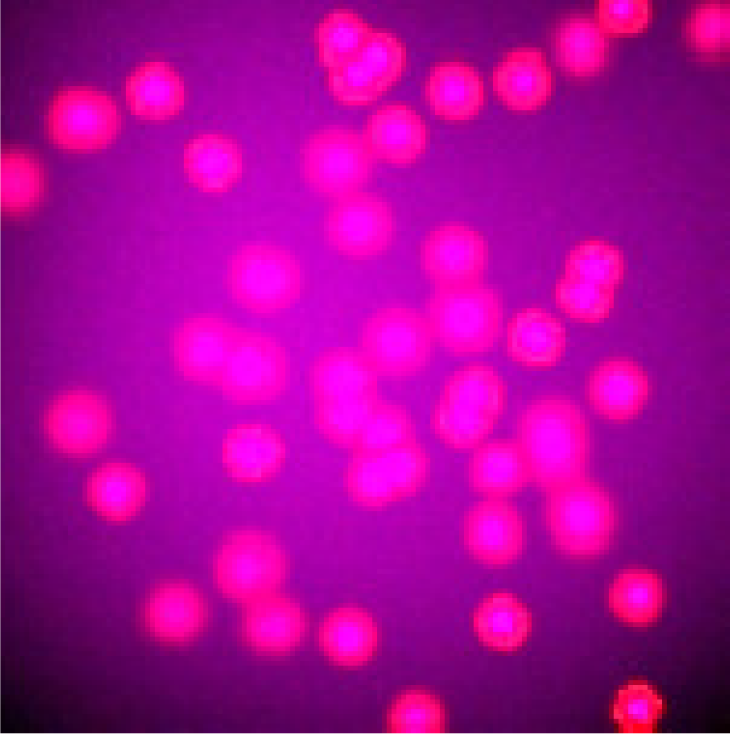
\includegraphics[scale=0.35]{FluoCell.png}
  \caption{Tratto da \cite{guberman2016complex}. Immagini simulate al computer di cellule fluorescenti che la rete neurale convoluzionale a valori complessi deve identificare.}
  \label{FluoCellpng}
 \end{figure}
 
 I risultati ottenuti sono molto buoni e promettenti: infatti anche se l'accuratezza sul set di test \'e praticamente uguale tra rete a valori reali e rete a valori complessi (tabella \ref{FluoAccuracyTab}), le reti a valori complessi soffrono meno di overfitting.
 \begin{table}[h]
  \centering
  \begin{tabular}{|c|c|c|c|c|}
   \hline
    & Train loss & Train accuracy & Test loss & Test Accuracy \\
    \hline
    Complex network & 0.056 & 97.4\% & 0.069 & 97.3\% \\
    \hline
    Real network & 0.007 & 99.8\% & 0.145 & 97.5\% \\
    \hline
  \end{tabular}
  \caption{Tratto da \cite{guberman2016complex}. Risultati del modello reale e di quello complesso nel set di trining e di test. Si noti come il test loss della rete reale sia decisamente maggiore rispetto a quello della rete complessa.}
 \end{table}

 Ci\'o viene mostrato ancora meglio nel confronto effettuato nei grafici \ref{FluoConvergapng} e \ref{FluoConvergbpng} della convergenza delle due reti in funzione del numero delle epochs (per ogni epoch viene effettuato un determinato numero di cicli di train e di test per determinare l'accuratezza).
 \begin{figure}[h!]
  \centering
  \begin{subfigure}[b]{\linewidth}
   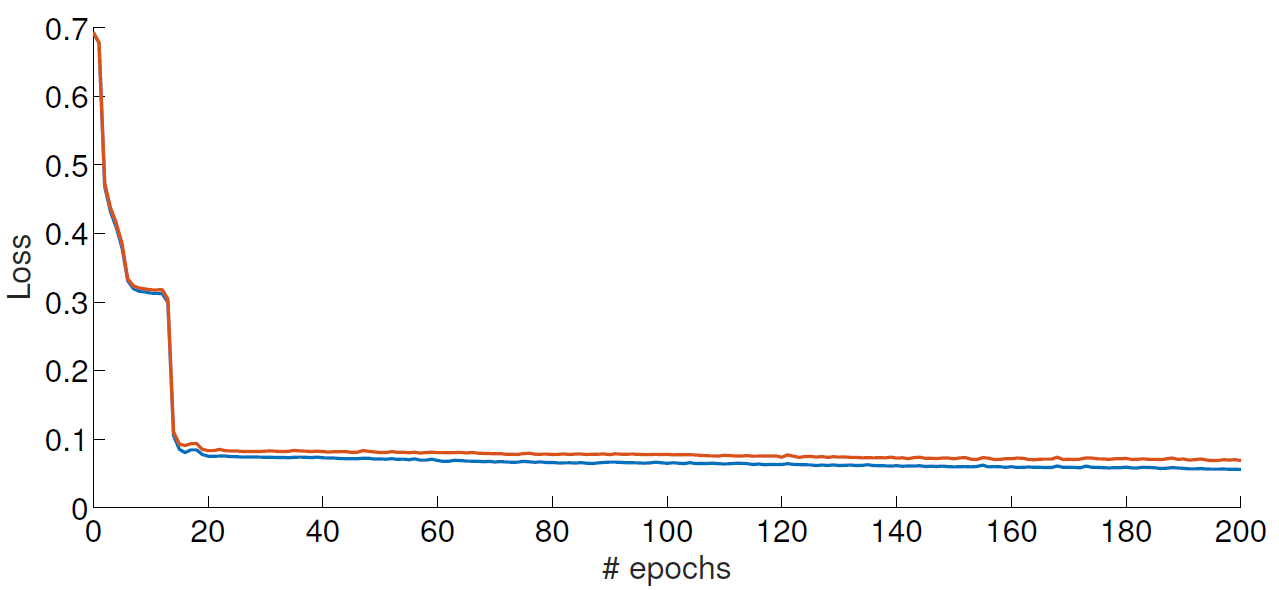
\includegraphics[scale=0.5]{FluoConverga.png}
   \caption{Tratto da \cite{guberman2016complex}. Convergenza della rete neurale a valori complessi.}
   \label{FluoConvergapgn}
  \end{subfigure}
  \\
  \begin{subfigure}[b]{\linewidth}
   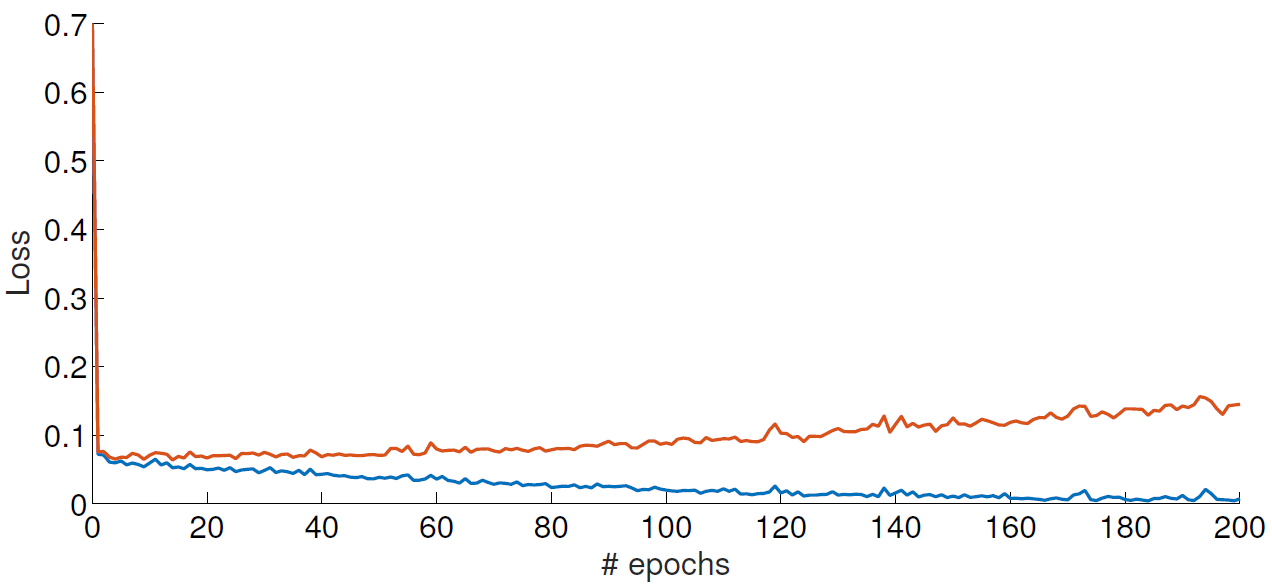
\includegraphics[scale=0.5]{FluoConvergb.png}
   \caption{Tratto da \cite{guberman2016complex}. Convergenza della rete neurale a valori reali.}
   \label{FluoConvergbpgn}
  \end{subfigure}
  \caption{Convergenza delle reti reali e complesse in funzione dei progressi dell'algoritmo. Una epoch \'e il numero di iterazioni in cui il numero totale di esempi scelti \'e uguale alla dimensione dell'insieme di addestramento, in questo caso una epoch \'e di 100 iterazioni. Nella linea blu, la funzione di loss dell'allenamento e nella linea rossa quella del test. Il modello reale soffre di overfitting, mentre il complesso no.}
 \end{figure}
 
 Bisogna tenere a mente che in \cite{guberman2016complex} viene esplicitata la scelta di confrontare solo i risultati migliori e suppongo che anche per gli altri dati ottenuti sia stata fatta la stessa scelta.
 Per\'o in \cite{guberman2016complex} si ha la possibilit\'a di capire cosa significhi questa scelta: in figura \ref{FluoConvergAttemptspng} viene mostrato come solo 4 volte su 20 la rete riesce a raggiungere la convergenza desiderata.
 \begin{figure}[h]
  \centering
  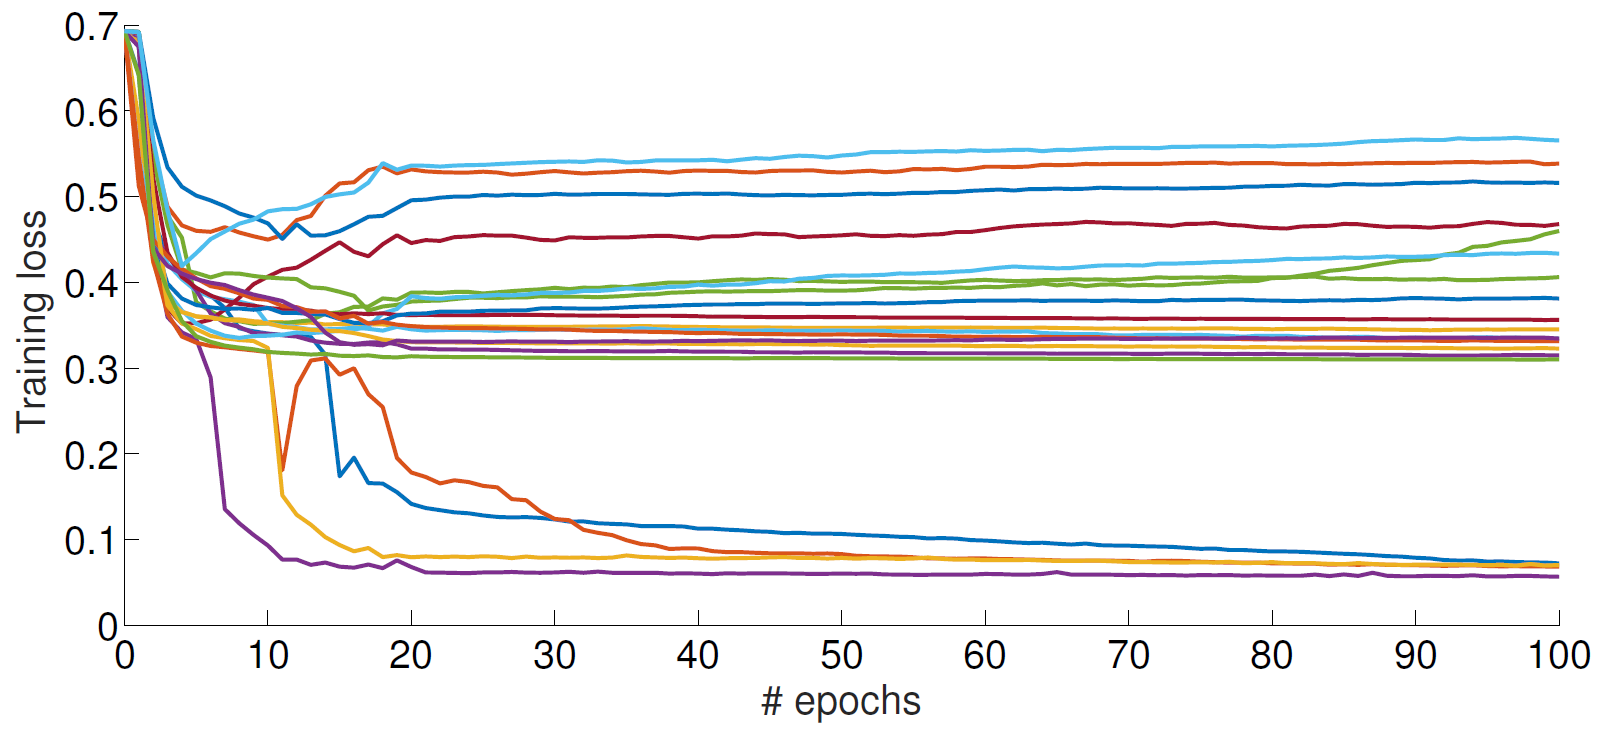
\includegraphics[scale=0.4]{FluoConvergAttempts.png}
  \caption{Tratto da \cite{guberman2016complex}. Training ripetuto della rete complessa. Ogni riga rappresenta il training loss in tutte le epochs di una singola prova. Il tasso di apprendimento \'e ridotto dopo 20 epochs, per una convergenza ottimale. Il processo di allenamento \'e instabile e sensibile agli effetti di randomizzazione. Non tutte le prove sono convergenti e, tra queste, la maggior parte non ha raggiunto il minimo globale.}
 \end{figure}

 
 Per poter migliorare questo aspetto, di seguito trattato metodi per poter migliorare la resistenza all'overfitting, ma, ancor pi\'u importante, migliorare la generalizzazione e la ricerca del minimo globale della rete neurale.



 



 
 \chapter*{Ottimizzazione}
 \section{ensemble di reti neurali}
 Una rete di dimensioni finite raramente apprende completamente un particolare mapping e pu\'o generalizzare male. Aumentare la dimensione o il numero di hidden layer per\'o, il pi\'u delle volte, non porta a nessun miglioramento \cite{soulie1987evaluation} anzi, aumentando la dimensionalit\'a del problema aumenta la possibilit\'a che la rete si stabilizzi lontana dalla soluzione desiderata. 
 Molti ricercatori hanno dimostrato che la semplice combinazione degli output di molti classificatori pu\'o generare previsioni pi\'u accurate di quelle di qualsiasi classificatore \cite{clemen1989combining} \cite{wolpert1992stacked}. In particolare, la combinazione di reti neurali addestrate separatamente (comunemente indicato come ensemble di reti neurali) si \'e dimostrata particolarmente efficace \cite{alpaydin1993multiple} \cite{drucker1994boosting} \cite{krogh1995neural} \cite{maclin1995combining} \cite{perrone1992soft}. 
 Figura \ref{EnsembleStructurepng} illustra la struttura generale di un ensemble di reti neurali. Ogni rete nell'ensemble \'e per prima cosa addestrata e poi, per ogni esempio del training, l'output predetto di ognuna delle reti \'e combinato dal judge per produrre l'output dell'ensemble. 
 \begin{figure}[h!]
  \centering
  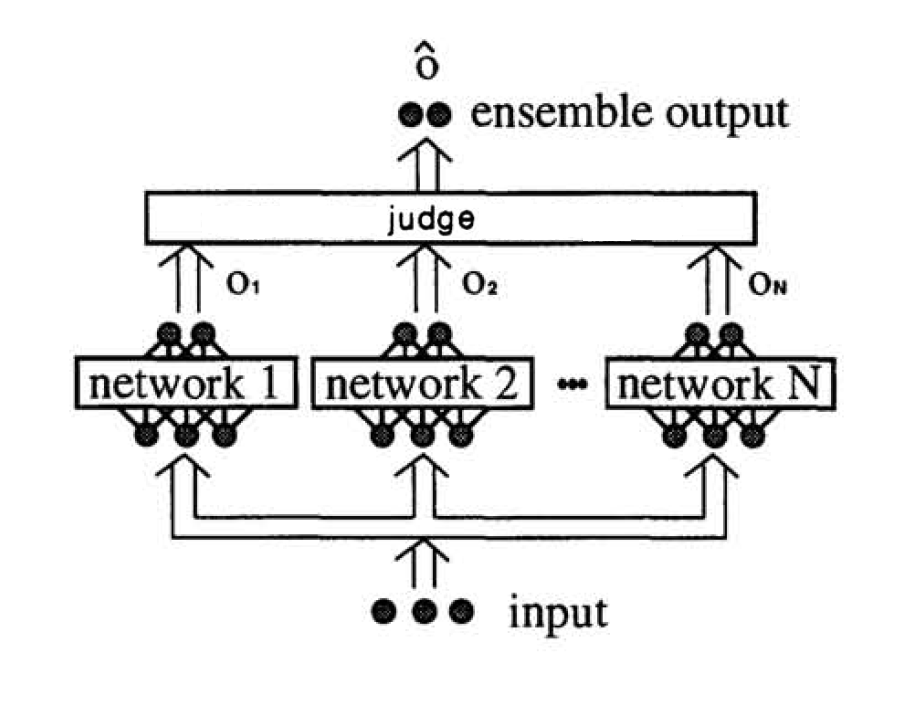
\includegraphics[scale=0.4]{EnsembleStructure.png}
  \caption{Struttura di un ensemble di reti neurali. In basso l'input in comune per tutte le reti. Gli output di queste ultime viene poi combinato dal judge attraverso i pesi $w_1, \cdots , w_N$.}
  \label{EnsembleStructurepng}
 \end{figure}
 
 L'output dell'ensemble pu\'o anche essere utilizzato come ulteriore training restituendolo alle singole reti. 
 Infatti, nel caso in cui nell'ensemble vi siano una o pi\'u reti poco efficienti e non si hanno a disposizione pi\'u esempi per il training, si pu\'o utilizzare l'output dell'ensemble come output desiderato nelle singole reti per continuare l'addestramento \cite{lincoln1990synergy}. 
 
 L'errore di una singola rete dipende dalle dimensioni dell'hidden layer e dalla durata del training. 
 Tuttavia in generale l'errore non \'e una funzione decrescente della dimensione dell'hidden layer. 
 In figura \ref{NetErrHiddenLapng} e \ref{NetErrHiddenLbpng} si mostra l'errore di una singola rete rispetto alla dimensione dell'hidden layer riscontrato da \cite{lincoln1990synergy} per diversi step di training. 
 D'altra parte la miglior capacit\'a di apprendimento di un ensemble dipende, come accennato in precedenza, dalla sinergia tra le singole reti e non dalle maggiori dimensioni rispetto alla singola rete. 
 In \cite{lincoln1990synergy} vengono confrontate le prestazioni di ogni singola rete con le prestazioni di un enseble di 5 reti neurali, con stessa struttura della singola.
 
 \begin{figure}[h!]
  \centering
  \begin{subfigure}[b]{0.4\linewidth}
   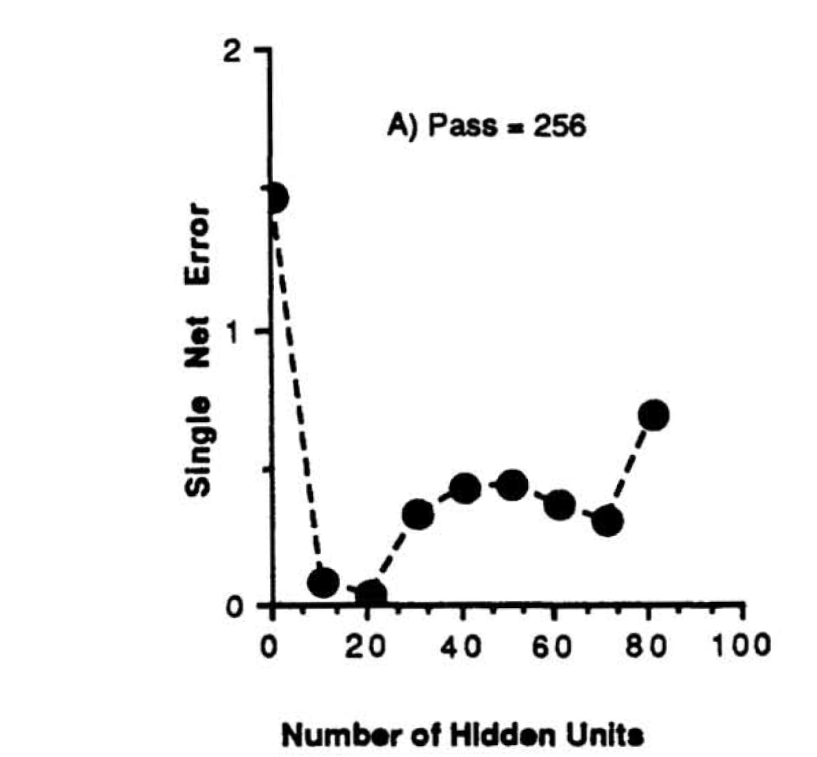
\includegraphics[width=\linewidth]{NetErrHiddenLa.png}
   \label{NetErrHiddLapgn}
  \end{subfigure}
  \begin{subfigure}[b]{0.4\linewidth}
   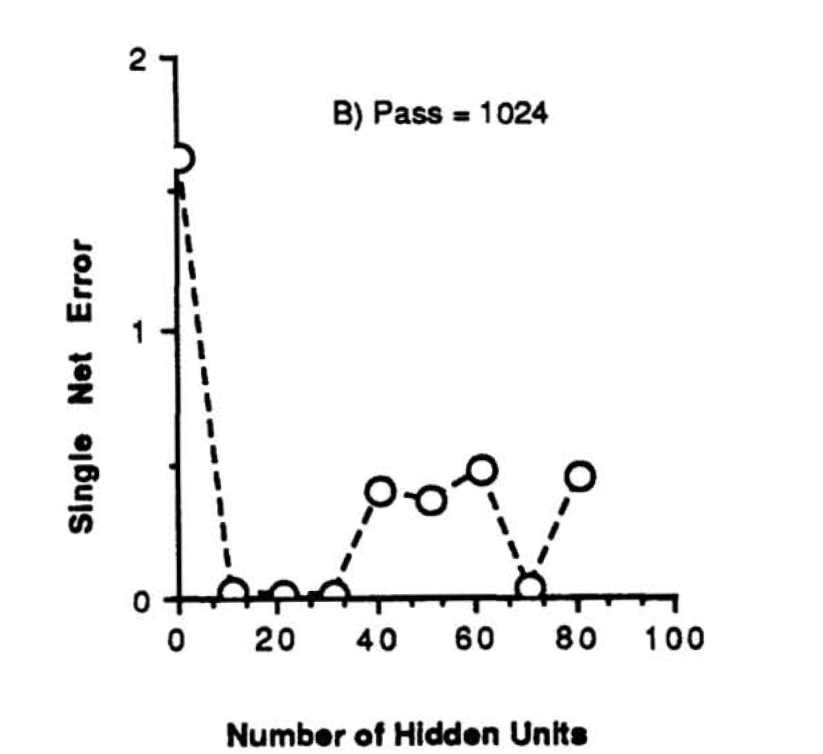
\includegraphics[width=\linewidth]{NetErrHiddenLb.png}
   \label{NetErrHiddLbpgn}
  \end{subfigure}
  \caption{Tratto da \cite{lincoln1990synergy}. Errore della singola rete in funzione del numero di hidden layer, in dimostrazione del fatto che la relazione non \'e lineare.}
 \end{figure}

 
 Vengono confrontati gli errori medi dei due sistemi. 
 Figura \ref{EnsembleAdvantageapng} e \ref{EnsembleAdvantagebpng} mostrano il vantaggio dell'ensemble rispetto agli errori della rete singola rispettivamente per 256 e 1024 step del training. 
 Nei casi estremi in cui l'apprendimento sia nullo o quasi totale, l'ensemble non mostra particolari vantaggi, tuttavia si ha un notevole vantaggio se l'apprendimento \'e solo parziale.
 
 \begin{figure}[h!]
  \centering
  \begin{subfigure}[b]{0.4\linewidth}
   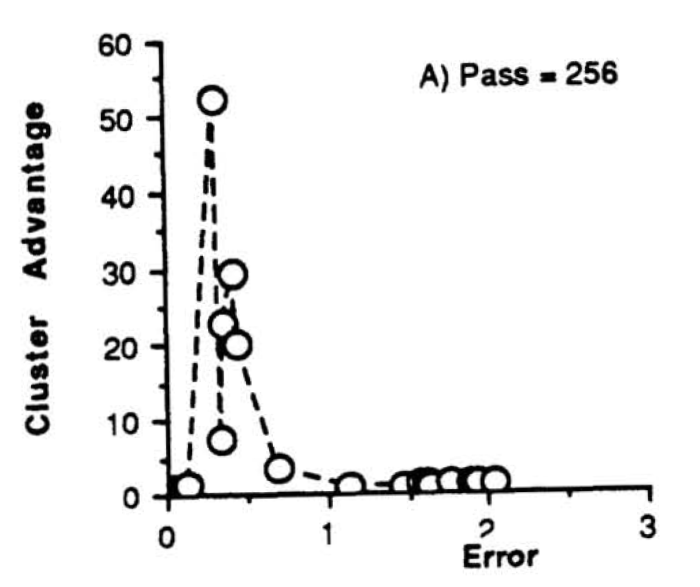
\includegraphics[width=\linewidth]{ClusterErrora.png}
   \label{EnsembleAdvantageapng}
  \end{subfigure}
  \begin{subfigure}[b]{0.4\linewidth}
   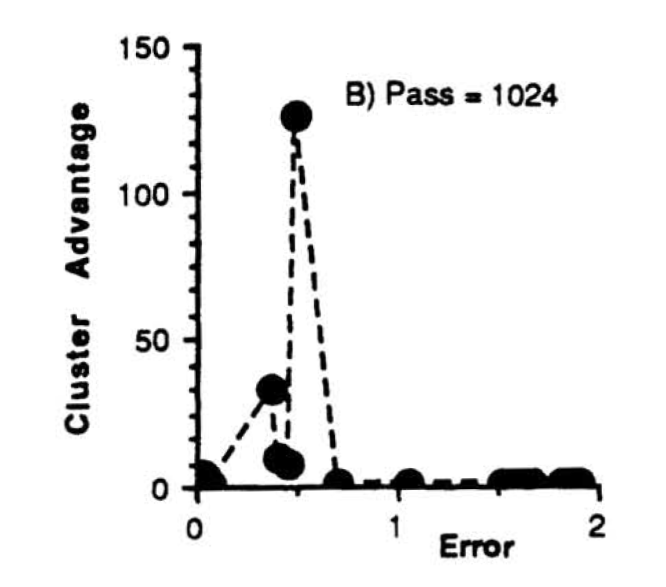
\includegraphics[width=\linewidth]{ClusterErrorb.png}
   \label{EnsembleAdvantagebpng}
  \end{subfigure}
  \caption{Tratto da \cite{lincoln1990synergy}. Vantaggio del cluster in funzione dell'errore. A) dopo 256 step del training e B) dopo 1024 step del training.}
 \end{figure}
 
 \subsection{judge}
 
 Dato un singolo input, le reti neurali dell'ensemble daranno presumibilmente degli output $Y_k$ diversi, che diventano l'input del $judge$. Quest'ultimo combinandoli ottiene il risultato finale $Y$. 
 Esistono diversi metodi per calcolare $Y$, ma per semplicit\'a consideriamo i due casi pi\'u semplici:
 \begin{align}
  Y &= \sum_{k=1}^N \frac{1}{N} Y_k \\
  Y &= \sum_{k=1}^N W_k Y_k
 \end{align}
 Il primo \'e dato da una semplice media dei $Y_k$, mentre nel secondo caso si considera una media pesata, con i $W_k$ che indicano ``l'affidabilit\'a'' delle singole reti neurali. 
 Seguendo questo ragionamento i $W_k$ vengono di volta in volta modificati come segue:
 \begin{align}
  W_k &= W_k \cdot G \cdot \frac{e}{e_k} \label{JudgeWeights} \\
  e &= \frac{1}{N} \sum{k=1}^N e_k \\
  e_k &= \left | Y - Y_k \right |
 \end{align}
 Con $e$ che indica il tasso di correzione e $e_k$ \'e la deviazione dell'output della singola rete dall'output dell'ensemble.
 
 Dopo il periodo di training iniziale, si presume generalmente che la rete neurale non sia pi\'u soggetta ad ulteriore training. 
 Tuttavia, come gi\'a anticipato, si pu\'o restituire l'output del judge alle singole reti neurali come output desiderato. 
 William P. Lincoln e Josef Skrzypek in \textit{Synergy of clustering multiple back propagation networks} affermano che questo procedimento migliori la resistenza al rumore e l'auto-organizzazione $(da capire cosa sia)$.
  
 \subsection{ottimizzazione dell'ensemble}
  Precedenti lavori sia teorici \cite{hansen1990neural} \cite{krogh1995neural} che empirici \cite{hashem1994optimal} \cite{maclin1995combining} hanno dimostrato che un ensemble efficace dovrebbe consistere non solo in reti particolarmente performanti, ma anche in reti che commettano errori in parti distinte dello spazio degli input. 
 
 Assumiamo che l'obiettivo sia quello di apprendere una funzione $f:R^N\to R$ per la quale abbiamo $p$ coppie input-output per il training con $Y_k = f \left( x_k \right) $ e $k=1, \cdots , p$. 
 L'ensenble consiste in $N$ reti e chiamiamo $V^{\alpha}\left( x\right)$ l'output della rete $\alpha$ relativo all'input $x$. 
 Definiamo nel modo seguente il valore ottenuto dal judge: 
  \begin{equation}
   \overline{V}\left(x\right) = \sum_{\alpha} w_{\alpha} V^{\alpha}\left(x\right).
  \end{equation}
  Consideriamo i pesi $w_{\alpha}$ come l'affidabilit\'a della rete $\alpha$ e di conseguenza li vincoliamo ad essere positivi e normalizzati, cio\'e $\sum_{\alpha} w_{\alpha} = 1$. 
  L'\textit{ambuiguit\'a} su un input $x$ di un singolo membro dell'ensemble \'e definito come $a^{\alpha}\left(x\right)=\left(V^{\alpha}\left(x\right)-\overline{V}\left(x\right)\right)^2$. 
  La \textit{ambiguit\'a dell'ensemble} su un input $x$ \'e data da:
  \begin{equation}
   \overline{a}\left(x\right) = \sum_{\alpha} w_{\alpha} a^{\alpha}\left(x\right) = \sum_{\alpha} w_{\alpha}\left(V^{\alpha}\left(x\right)-\overline{V}\left(x\right)\right)^2. \label{EnsembleAmbiguity}
  \end{equation}
  \'E quindi una varianza e misura il disaccordo delle reti sull'input $x$. 
  L'errore quadratico della rete $\alpha$ e dell'ensemble sono rispettivamente:
  \begin{align}
   e^{\alpha}\left(x\right) &= \left(f\left(x\right)-V^{\alpha}\left(x\right)\right)^2 \\
   e\left(x\right) &= \left(f\left(x\right)-\overline{V}\left(x\right)\right)^2 \label{ensembleQE}
  \end{align}
  Aggiungendo e sottraendo $f\left(x\right)$ alla \ref{EnsembleAmbiguity} si ottiene:
  \begin{equation}
   \overline{a}\left(x\right) = \sum_{\alpha} w_{\alpha} e^{\alpha}\left(x\right) - e\left(x\right).
  \end{equation}
  Chiamando la media pesata degli errori delle singole reti $\overline{e}\left(x\right) = \sum_{\alpha} w_{\alpha} e^{\alpha}\left(x\right)$ allora la \ref{ensembleQE} diventa:
  \begin{equation}
   e\left(x\right) = \overline{e}\left(x\right) - \overline{a}\left(x\right). \label{GeneralizationError}
  \end{equation}
  Queste ultime formule possono essere mediate lungo la distribuzione degli input, ottenendo le seguenti:
  \begin{align}
   E^{\alpha} &= \int dx \; p\left(x\right) \; e^{\alpha}\left(x\right) \\
   A^{\alpha} &= \int dx \; p\left(x\right) \; a^{\alpha}\left(x\right) \\
   E &= \int dx \; p\left(x\right) \; e\left(x\right).
  \end{align}
  Le prime due sono rispettivamente l'errore generalizzato e l'ambiguit\'a della rete $\alpha$ e $E$ \'e l'errore generalizzato dell'ensemble. 
  Dalla \ref{GeneralizationError} otteniamo:
  \begin{equation}
   E = \overline{E} - \overline{A} \label{EnsembleGeneralizationError}
  \end{equation}
  con $\overline{E} = \sum_{\alpha} w_{\alpha} E^{\alpha}$ la media pesata degli errori generalizzati delle singole reti e $\overline{A} = \sum_{\alpha} w_{\alpha} A^{\alpha}$ la media pesata delle ambiguit\'a delle singole reti.
  
  Questa equazione separa l'errore generalizzato in un termine che dipende dagli errori generalizzati delle singole reti e da un altro contenente le correlazioni tra le reti. 
  Inoltre, il termine di correlazione $A$ pu\'o essere stimato interamente da dati non etichettati, non \'e richiesta alcuna conoscenza della funzione da approssimare. 
  Il termine ``senza etichetta'' \'e tratto dai problemi di classificazione e in questo contesto si riferisce a un input $x$ per il quale non si conosce il valore $f(x)$ della funzione target. 
  Se l'ensemble \'e fortemente distorto, l'ambiguit\'a sar\'a piccola, perch\'e le reti implementano funzioni molto simili e concordano quindi gli input anche al di fuori del training. 
  Pertanto l'errore generalizzato sar\'a sostanzialmente uguale alla media degli errori delle singole reti. 
  Se, d'altra parte, c'\'e una grande varianza, l'ambiguit\'a \'e alta e in questo caso l'errore di generalizzazione sar\'a pi\'u piccolo dell'errore di generalizzazione medio.
  Vediamo immediatamente che l'errore generalizzato dell'ensemble \'e sempre minore della media pesata degli errori degli ensemble: $E < \overline{E}$. In particolare, per pesi uniformi:
  \begin{equation}
   E \le \frac{1}{N} \sum_{\alpha} E^{\alpha}
  \end{equation}
  Dalla \ref{EnsembleGeneralizationError} si ricava che aumentare l'efficienza dell'ensemble significa aumentare l'ambiguit\'a e quindi la discordanza tra le reti singole senza aumentarne ovviamente l'errore generalizzato. 
  Come aumentare l'ambiguit\'a dell'ensemble? Un metodo pu\'o essere quello di utilizare diverse tipologie di reti neurali, oppure di utilizzare set di training diversi. 
  Inoltre, per essere in grado di stimare il primo termine in \ref{EnsembleGeneralizationError}, sarebbe auspicabile una cross-validation. 
  In \cite{krogh1995neural} viene testato questo metodo per approssimare con un ensemble di reti neurali un'onda quadra in una variabile, mostrata in figura \ref{SqWavepng}. 
  Sono state utilizzate 5 reti con un hidden layer di 20 ``neuroni'', addestrate indipendenemente le une dalle altre mediande back-propagation utilizzando 200 esempi casuali. 
  L'ambiguit\'a \'e stata stimata da un insieme di 1000 input e i pesi associati agli output delle singole reti per la combinazione erano uniformi $w_{\alpha} = 1/5$.
  \begin{figure}[h!]
   \centering
   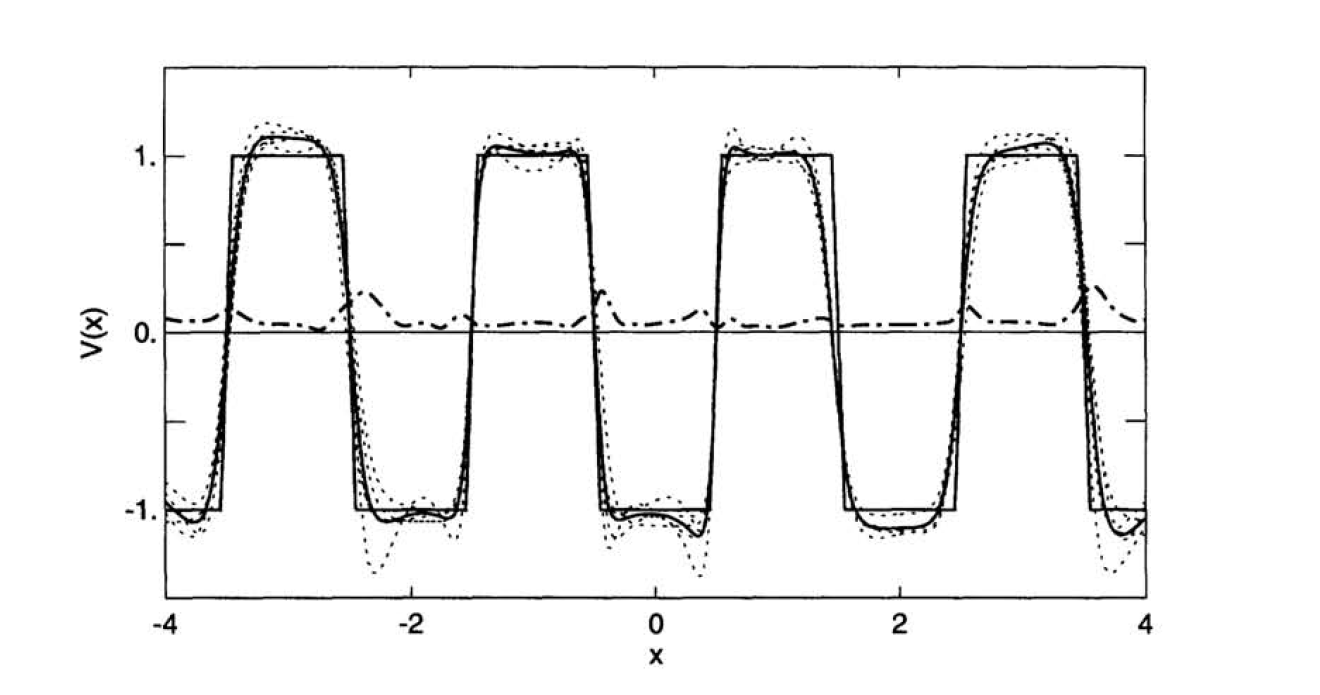
\includegraphics[scale=0.4]{SqWave.png}
   \caption{Tratto da \cite{krogh1995neural}. La linea spessa e continua indica l'output dell'ensemble, mentre quelle tratteggiate gli output delle singole reti. Viene mostrata anche l'ambiguit\'a (dash-dot line).}
   \label{SqWavepng}
  \end{figure}
  In figura \ref{GenErrorpng} viene mostrato l'errore generalizzato in funzione della dimensione $K$ dei set per la cross-validation.
  \begin{figure}[h!]
   \centering
   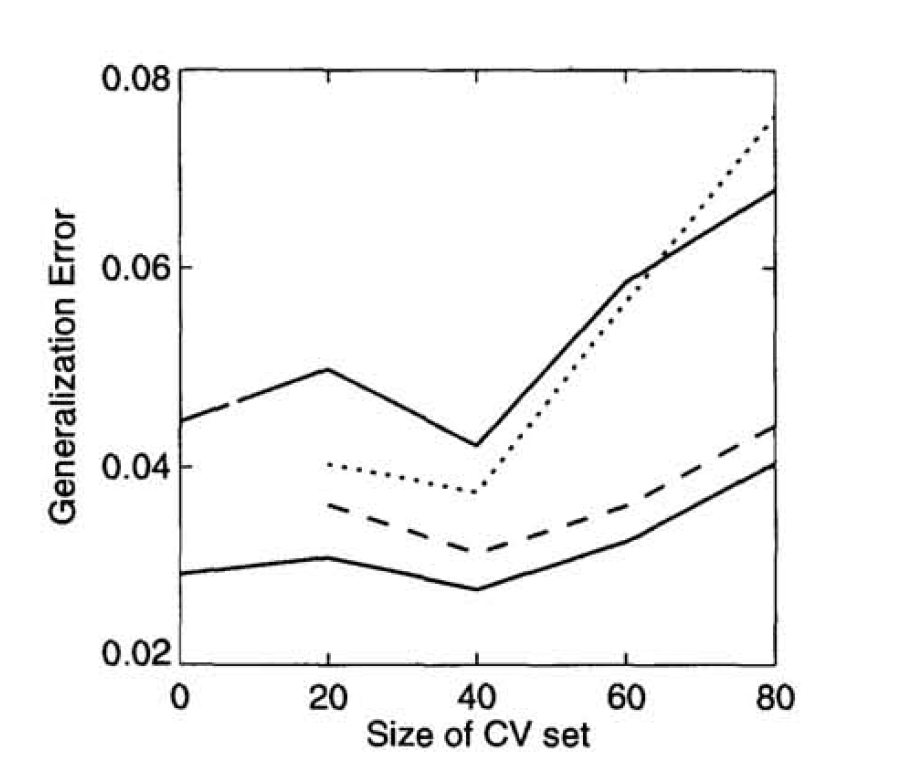
\includegraphics[scale=0.4]{GenError.png} 
   \caption{Tratto da \cite{krogh1995neural}. La linea continua mostra l'errore generalizzato per pesi uniformi in funzione di $K$, dove $K$ \'e la dimensione dei set di convalida. La linea tratteggiata \'e l'errore stimato dall'equazione \ref{EnsembleGeneralizationError}. La linea tratteggiat \'e per i pesi ottimali stimati dall'uso degli errori di generalizzazione per le singole reti, stimate dai set di crossvalidation. La linea continua inferiore \'e l'errore generalizzato che si otterrebbe se i singoli errori di generalizzazione fossero conosciuti esattamente.}
   \label{GenErrorpng}
  \end{figure}
  Innanzitutto notiamo come l'errore generalizzato sia lo stesso per un set di cross-validation di dimensione 40 o 0. 
  Tuttavia bisogna considerare che sono stati scartati tutti i risultati di ensemble con due o pi\'u reti non convergenti.

  Dopo aver definito pi\'u chiaramente il problema da affrontare, cerchiamone una soluzione. 
  La maggior parte dei lavori \'e concentrata sulla combinazione degli output di reti pi\'u performanti o ha indirizzato solo indirettamente il modo in cui generare un buon ensemble di reti, generando casualmente diverse topologie, impostazioni iniziali dei pesi, dei parametri o utilizzando solo una parte del set di training nella speranza di produrre reti che commettano errori per input distinti. 
  Per trovare direttamente un ensemble accurato e diversificato si possono sfruttare gli algoritmi genetici, creando una popolazione iniziale e utilizzando operatori genetici per creare continuamente nuove reti, mantenendo di volta in volta solo l'insieme di reti pi\'u performanti e al contempo pi\'u discordi tra loro. 

  
  Di seguito sintetizziamo l'algoritmo utilizzato. 
  Viene creata una popolazione iniziale di reti neurali sottoposta a training. 
  Di seguito si creano nuove reti partendo dalle precedenti utilizzando operazioni ``genetiche'' come mutazioni e crossover. 
  La nuova popolazione viene nuovamente addestrata, ponendo particolare attenzione ad utilizzare gli esempi classificati erroneamente dalla popolazione precedente. 
  Viene quindi associato un punteggio determinato dalla funzione di fitness:
  \begin{equation}
   Fitness_i = Accuracy_i + \lambda Diversity_i = (1-E_i) + \lambda D_i \label{fitness}
  \end{equation}
  con la diversit\'a definita come:
  \begin{equation}
   D_i = \sum \left[ V_i \left(x\right) - \overline{V} \left(x\right) \right]^2. \label{diversity}
  \end{equation}
  
  Definiamo il termine di accuratezza del set di convalida della rete come $A_i = 1-E_i$ e utilizziamo l'equazione \ref{diversity} per calcolare il termine di diversit\'a $D_i$. 
  Quindi normalizziamo separatamente ciascuno dei due termini. Non essendo sempre chiaro con quale valore si debba settare $\lambda$, solitamente ci si basa sulle seguenti regole. 
  Il valore di $\lambda$ non si modifica se l'errore dell'ensemble $\widehat{E}$ diminuisce mentre consideriamo nuove reti. 
  Cambia invece se si verifica una delle seguenti: (1) se l'errore della popolazione $\overline{E}$ non sta aumentando e la diversit\'a $D$ sta diminuendo, aumentiamo $\lambda$; (2) se $\overline{E}$ sta aumentando e $\overline{D}$ non decresce, caliamo $\lambda$.
  
  Tabella \textbf{GOAL:} creare geneticamente un ensemble di reti accurate e diversificate.
  \begin{itemize}
   \item Creare e addestrare la popolazione iniziale di reti.
   \item Finch\'e non si raggiunge un limite di efficacia o di tempo:
   \begin{itemize}
    \item Utilizzare operazioni genetiche per creare nuove reti.
    \item Addestrare le nuove reti utilizzando l'equazione \ref{EnsembleCostFunc}.
    \item Misurare la diversit\'a di ogni rete rispetto alla popolazione corrente (equazione \ref{diversity}).
    \item Normalizzare i termini di accuratezza e diversit\'a delle singole reti.
    \item Cacolare la funzione di fitness in equazione \ref{fitness}.
    \item Aggiornare la popolazione utilizzando le $N$ reti con valore maggiore per la \ref{fitness}.
    \item Corregere $\lambda$ dell'equazione \ref{fitness}
    \item Utilizzare la popolazione attuale di reti come ensemble e combinare gli output delle reti seguendo l'equazione \ref{JudgeWeights}
   \end{itemize}
  \end{itemize}
  Ribadiamo che una rete utile all'ensemble \'e quella che classifica correttamente il maggior numero possibile di casi, mentre pecca principalmente laddove le altre reti classificano correttamente. 
  Ci preoccupiamo di questo aspetto durante la backpropagation moltiplicando la normale funzione di costo per un termine che misura l'errore combinato della popolazione su un determinato esempio:
  \begin{equation}
   Cost = \sum_{k \in T} \left| \frac{t \left(k\right) - \widehat{o} \left(k\right)}{\widehat{E}} \right|^{\frac{\lambda}{\lambda + 1}} \left[ t\left(k\right) - a\left(k\right) \right]^2 \label{EnsembleCostFunc}
  \end{equation}
  dove $t(k)$ \'e il target e $a(k)$ \'e l'attivazione della rete per l'esempio k nel training set $T$. 
  Si noti che, dato che la nostra rete non \'e ancora un membro dell'ensemble, $\widehat{o} (k)$ e $\widehat{E}$ non dipendono dalla nostra rete; il nuovo termine \'e perci\'o una costante quando calcoliamo le derivate nella back propagation. 
  Normalizziamo $t(k) - \widehat{o} (k)$ dividendo per l'errore dell'ensemble $\widehat{E}$ in modo che il valore medio del nostro nuovo termine sia circa 1 indipendentemente dalla correttezza dell'insieme. 
  Ci\'o \'e particolarmente importante con popolazioni particolarmente accurate, poich\'e $t(k) - \widehat{o} (k)$ sar\'a vicino a 0 per la maggior parte degli esempi e la rete verrebbe addestrata solo su un numero esiguo di esempi. 
  L'esponenete $\frac{\lambda}{\lambda + 1}$ rappresenta il rapporto di importanza del termine di diversit\'a nella funzione di fitness. 
  Ad esempio, se $\lambda$ \'e vicino a 0, la diversit\'a non \'e considerata importante e la rete viene addestrata con la consueta funzione di costo; tuttavia se $\lambda$ \'e grande, la diversit\'a \'e cosiderata importante e il nuovo termine nella funzione di costo assume maggiore importanza. 
  Combiniamo le previsioni delle reti prendendo una somma ponderata dell'output di ciascuna rete, dove ogni peso \'e definito come in precedenza. Riportiamo di seguito i risultati ottenuti da David W. Opitz e Jude W. Shavlik \cite{opitz1994using}.
  
  L'algoritmo genetico che viene utilizzato per generare nuove topologie di rete \'e l'algoritmo REGENT \cite{opitz1994using}. 
  REGENT utilizza algoritmi genetici per effettuare ricerche nello spazio delle topologie della rete neurale KN. 
  I KN sono reti le cui topologie sono determinate a seguito della mappatura diretta di un insieme di regole di base che rappresentano ci\'o che attualmente si conosce del problema da affrontare. 
  KBANN \cite{towell1994knowledge}, per esempio, traduce un insieme di regole proposizionali in una rete neurale, quindi affina i pesi della rete risultante usando la back-propagation. L'uso di KNN consente di avere reti altamente corrette nell'ensemble; tuttavia, poich\'e ogni rete nell'ensemble \'e inizializzata con lo stesso insieme di regole specifiche del dominio, non ci si aspetta che vi sia un grande disaccordo tra le reti. 
  Un'alternativa da considerare \'e quella di generare casualmente la opolazione iniziale di topologie di rete, poich\'e a volte le regole specifiche del dominio non sono disponibili.
  \'E stato eseguito l'algoritmo genetico sul set di problemi MAX di NYNEX e su tre problemi del progetto genoma umano che aiutano a localizzare i geni nelle sequenze di DNA. 
  Ognuno di questi domini \'e accompagnato da una serie di regole approssimativamente corrette che descrivono ci\'o che attualmente \'e noto su tale attivit\'a \cite{opitz1995anytime} \cite{opitz1994using}. 
  Gli esperimenti misurano l'errore del set di test dell'algoritmo genetico su queste attivit\'a. 
  Ogni ensemble \'e composto da 20 reti e gli algoritmi REGENT e ADDEMUP (cos\'i \'e stato chiamato l'algoritmo genetico utilizzato in \cite{opitz1996generating}) hanno considerato 250 reti durante la loro ricerca genetica. La tabella \ref{NoKnowledgeTab} presenta i risultati del caso in cui si crei casualmente la topologia delle reti. 
  La prima riga della tabella \ref{NoKnowledgeTab}, la migliore rete, deriva da una rete neurale a singolo strato in cui, per ogni fold abbiamo addestrato 20 reti contenenti tra 0 e 100 hidden nodes e usato un set di validazione per scegliere la migliore. 
  La riga successiva, il bagging, contiene i risultati dell'esecuzione dell'algoritmo di bagging di Breiman \cite{breiman1994bagging} su reti standard con un unico hidden layer, in cui il numero di hidden nodes viene impostato casualmente tra 0 e 100 per ogni rete. 
  Il bagging \'e un ``bootstrap'', cio\'e un metodo dell'ensemble che forma ogni rete con una diversa partizione dell'insieme di addestramento. 
  Genera ogni partizione tracciando casualmente, con la sostituzione, N esempi dal set di addestramento, dove N \'e la dimensione del set di addestramento. 
  Breiman (1994) \cite{breiman1994bagging} ha dimostrato che il bagging \'e efficace su algoritmi di apprendimento ``instabili'', come le reti neurali, in cui piccoli cambiamenti nel set di addestramento comportano grandi cambiamenti nelle previsioni. La riga inferiore della tabella \ref{NoKnowledgeTab}, ADDEMUP, contiene i risultati di una serie di ADDEMUP in cui la popolazione iniziale di 20 individui viene generata casualmente. 
  I risultati mostrano che su questi domini la combinazione dell'output di pi\'u reti addestrate di generalizza meglio rispetto al tentativo di scegliere la rete singola rete migliore. 
  Mentre la tabella \ref{NoKnowledgeTab} mostra la potenza degli insiemi di reti neurali, la tabella \ref{KnowledgeTab} mostra la capacit\'a di ADDEMUP di utilizzare le conoscenze a priori del problema. 
  La prima riga della tabella \ref{KnowledgeTab} contiene i risultati di generalizzazione dell'algoritmo KBANN, mentre la riga successica, KBANN-bagging, contiene i risultati dell'ensemble in cui ogni singola rete \'e la rete KBANN addestrata su una diversa partizione dell'insieme di addestramento. 
  Sebbene ciascuna di queste reti inizi con la stessa topologia e impostazione di peso iniziali ``grande'' (i pesi risultanti dalla conoscenza specifica del dominio), piccoli cambiamenti nel set di allenamento producono ancora cambiamenti significativi nelle previsioni. 
  Si noti inoltre che su tutti i set di dati, il bagging KBANN \'e migliore dell'esecuzione del bagging su reti generate casualmente (bagging della tabella \ref{NoKnowledgeTab}). 
  La riga successiva, REGENT-combined, contiene i risultati della semplice combinazione, usando l'equazione \ref{JudgeWeights}, degli output delle reti nella popolazione finale di REGENT. 
  ADDEMUP, l'ultima riga della tabella \ref{KnowledgeTab}, differisce principalmente da REGENT-combined in due modi: (1) la sua funzione di fitness (equazione \ref{fitness} ) tiene conto della diversit\'a piuttosto che della sola precisione della rete e (2) allena le nuove reti enfatizzando gli esempi errati dell'ensemble attuale. 
  Pertanto, il confronto di ADDEMUP con REGENT-combined aiuta a testare direttamente la diversit\'a di ADDEMUP, anche se i risultati aggiuntivi riportati in Opitz \cite{opitz1995anytime} mostrano che ADDEMUP ottiene gran parte del suo miglioramento dalla sua funzione di fitness. 
  Ci sono due ragioni principali per cui si ritiene che i risultati di ADDEMUP nella tabella \ref{KnowledgeTab} siano particolarmente incoraggianti: (1) confrontando ADDEMUP con REGENT-combined, \'e stata esplicitamente testata la qualit\'a dell'euristica e ne si dimostra l'efficacia e (2) ADDEMUP \'e in grado di utilizzare efficacemente le conoscenze di base per ridurre l'errore delle singole reti nel suo insieme, pur essendo in grado di creare abbastanza diversit\'a tra di loro in modo da migliorare la qualit\'a complessiva dell'ensemble. 
  
  \begin{table}[h]\caption{Tratto da \cite{opitz1994using}. Standard neural networks (no domain-specific knowledge used)} \label{NoKnowledgeTab}
   \centering
   \begin{tabular}[h]{|l|c|c|c|c|}
    \hline
    & Promoters & Splice Junction & RBS & MAX \\ \hline
   best-network & 6.6\% & 7.8\% & 10.7\% & 37.0\% \\ 
   bagging & 4.6\% & 4.5\% & 9.5\% & 35.7\% \\
   ADDEMUP & 4.6\% & 4.9\% & 9.0\% & 34.9\% \\ \hline
   \end{tabular}
  \end{table}
  
  \begin{table}[h]\caption{Tratto da \cite{opitz1994using}. Knowledge-based neural networks (domain-specific knowledge used)} \label{KnowledgeTab}
   \centering
   \begin{tabular}[h]{|l|c|c|c|c|}
    \hline
       & Promoters & Splice Junction & RBS & MAX \\ \hline
    KBANN & 6.2\% & 5.3\% & 9.4\% & 35.8\% \\ 
    KBANN-bagging & 4.2\% & 4.5\% & 8.5\% & 35.6\% \\
    REGENT-combined & 3.9\% & 3.9\% & 8.2\% & 35.6\% \\
    ADDEMUP & 2.9\% & 3.6\% & 7.5\% & 34.7\% \\ \hline
   \end{tabular}
  \end{table}


 \section{Funzione d'attivazione sticastica}
 La funzione d'attivazione gioca un ruolo fondamentale nel training delle rete neurali in quanto introduce la non linearit\'a indispensabile per poter approssimare una qualsiasi funzione. Tra le diverse descritte in precedenza ci concentriamo sulla ReLU, in particolare la funzione d'attivazione che sar\'a descritta prende in considerazione il valore ottenuto con la precedente e ci applica un rumore stocastico. In questo modo si riesce a prevenire meglio l'overfitting senza dover intervenire su quanto gi\'a appreso dalla rete durante il training. 
 Inizialmente si utilizzavano come funzione d'attivazione la sigmoide o la tangente iperbolica, in quanto continue, monotone e con condominio limitato. Il problema principale \'e dato dal fatto che le derivate tendono velocemente a valori molto piccoli, rallentando il processo di apprendimento. Per questo motivo la funzione ReLU \'e diventata particolarmente popolare e per comodit\'a la riprendiamo di seguito:
 \begin{equation} 
  ReLU\left(x\right) = max\left(x\right). 
 \end{equation} 
 La sua derivata  \'e data da:
 \begin{equation} 
  ReLU'\left(x\right) = \begin{cases} 
     1 & \mbox{se} \;\;\; x < 0 \\
     O & \mbox{altrimenti} 
 \end{cases} 
 \end{equation} 

 La ReLU risolve in parte il problema delle derivate, tuttavia si annulla per tutti i valori negativi producendo la "morte" del neurone. Per risolvere il problema sono state introdotte delle varianti della ReLU, come la Leaky ReLU\ref{LeakyReLU}. 
 L'idea di utilizzare una funzione di attivazione stocastica viene dal comportamento degli impulsi nervosi, i cui picchi sono disturbati da effetti bio-meccanici \cite{lewicki1998review}. La perturbazione indotta risulta essere particolarmente efficace nel prevenire l'overfitting durante il training. In particolare si introduce una nuova funzione d'attivazione il cui output produce una perturbazione stocastica; si propone poi un metodo per governare la perturbazione stocastica addestrando i parametri della distribuzione di probabilit\'a attraverso la back-propagation e viene mostrato come questa funzione d'attivazione aumenti le performance della rete, in particolare nell'ambito di "Visual object classification". 
 In figura \ref{ProbActEffectpng} visualizziamo i principali effetti dovuti all'applicazione di questa nuova funzione d'attivazione. 
 \begin{figure}[h!]
  \centering
  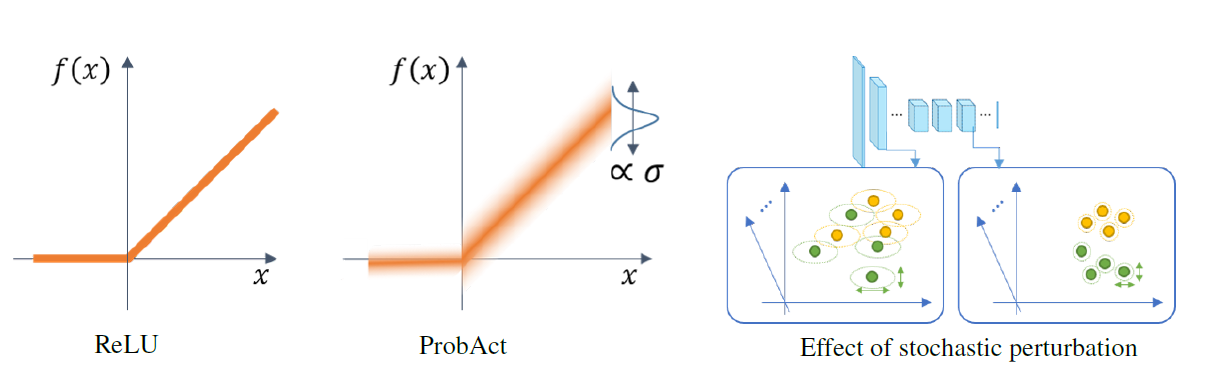
\includegraphics[scale=0.6]{ProbActEffect.png} 
  \caption{Confronto tra ReLU e funzione d'attivazione stocastica. L'effetto sfumato \'e stato introdotto solo per visualizzare come la funzione d'attivazione stocastica abbia come valore medio proprio $ReLU(x)$.}
  \label{ProbActEffectpng}
 \end{figure}
 
 In generale ogni layer di una rete neurale produce un output dato da:
 \begin{equation} 
  Y = f\left(w^{T} x\right), 
 \end{equation} 
 Dove $w^{T}$ indica il vettore dei pesi per quel layer, $x$ il vettore dell'input e $f$ la funzione d'attivazione, come pu\'o  essere la ReLU. Come mostrato in figura \ref{ProbActEffectpng} introduciamo una variabile randomica nella ReLU per creare una funzione d' attivazione stocastica. In particolare la si pu\'o definire come segue:
 \begin{equation} 
  f\left(x\right) = \mu \left(x\right) + z
 \end{equation} 
 Dove $\mu\left(x\right)$ \'e la ReLU e il tremine perturbativo $z$ pu\'o essere espresso come segue:
 \begin{equation} 
  z = \sigma  \epsilon. 
 \end{equation} 
 Il parametro perturbato $\sigma$ pu\' o essere fisso o addestrabile e definisce il range della perturbazione stocastica ed $\epsilon$ \'e il valore ottenuto dalla distribuzione normale. Studiamo i casi in cui $\sigma$ sia fissa o addestrata. 
 Nel caso sia fissa, ci sono diversi modi per definirne il valore pi\'u adatto. Scegliere una $\sigma$ costante per tutti i valori \'e una opzione valida poich\'e $\epsilon$ \'e ottenuta randomicamente da una distribuzione normale e $\sigma$ funge da fattore di scala. La rete \'e ottimizzata usando l'apprendimento basato sul gradiente definito dal seguente teorema:
 \newtheorem{teorema}{Teorema}
 
 \begin{teorema} \label{GradienPropth}
  La propagazione del gradiente di una unit\'a stocastica h basata su una funzione deterministica g con input x (vettore contenente gli output dagli altri neuroni) e parametri interni $\phi$ (pesi e bias); se il rumore z \'e possibile e se g(x,$\phi$ ,z) ha gradiente non nullo allora\\
  
  \centering
  h = g(x, $\phi$ , z)
 \end{teorema}


 La natura di $z$ \'e gaussiana, in quanto $z = \sigma \epsilon$ ed $\epsilon$ \'e effettivamente una variabile gaussiana. Ci\'o garantisce l'apprendimento attraverso il metodo basato sul gradiente. Il vantaggio principale di fissare $\sigma$ \'e quello di non aumentare il numero di parametri da dover addestrare nel training. 
 Si pu\'o comunque scegliere di lasciare $\sigma$ come parametro in pi\'u da addestrare durante il training tramite back-propagation, assieme agli altri parametri. Il calcolo del gradiente per $\sigma$ si ottiene attraverso la regola della catena. Data la funzione $F$, il gradiente di $F$ rispetto a $\sigma_{l, i}$ della $i$-esima unit\'a del $l$-esimo layer, \'e dato da:
 \begin{equation} 
  \frac{\partial F}{\partial\sigma_{l, i}} =  \frac{\partial F}{\partial y_{l, i}} \frac{\partial y_{l, i}}{\partial\sigma_{l, i}}
 \end{equation} 
 Con $y_{l, i}$ l'output dell'$i$-esima unit\'a del $l$-esimo layer. Il termine $\frac{\partial F}{\partial y_{l, i}}$ \'e il gradiente propagato dal layer pi\'u interno. Il gradiente dell' attivazione \'e dato da:
 \begin{equation} 
  \frac{\partial y_{l, i}}{\partial\sigma_{l, i}} = \epsilon
 \end{equation} 

 Addestrare $\sigma$ senza porre dei limiti pu\'o provocare l'annullamento o la divergenza del parametro perturbativo con conseguente difficolt\'a nel training. Sfruttando le propriet\'a della funzione sigmoide possiamo definire $\sigma = \alpha sigmoid(\beta k)$ per avere $\sigma$ confinata tra $0$ e $\alpha$. Con $k$ il parametro da imparare e $\alpha$ e $\beta$ parametri che posso essere tenuti fissi. Negli esperimenti descritti di seguito avremo $\alpha = 2$ e $\beta = 5$ (valori scelti dopo un test apposito). Figura \ref{ProbActEffectpng} illustra gli effetti della perturbazione stocastica. Intuitivamente, la funzione d'attivazione stocastica aggiunge perturbazioni ad ogni passaggio tra un layer e quello successivo in modo indipendente, funzionando cos\'i anche come regolarizzatore della rete. Bisogna ricordare che il rumore viene poi propagato in tutti i layer successivi, quindi il rumore totale aggiunto ad un certo layer dipende dal rumore applicato in precedenza, ma anche dai pesi. Ad esempio, anche nel caso pi\'u semplice in cui la rete abbia due layer con un ``neurone'' per ogni layer, la distribuzione dell'output $y_2$ del secondo layer differisce in base aai pesi del primo e secondo layer come segue:
 \begin{align}
  y_2 &= \mu \left[ w_2\mu\left(w_1 x\right) + w_2\sigma_1\epsilon\right] + \sigma_2\epsilon\\
  &= 
  \begin{cases}
   \mu\left[ w_2\mu\left(w_1 x\right)\right] + w_2\sigma_1\epsilon + \sigma_2\epsilon & \mbox{se} \;\; w_2\mu\left(w_1 x\right) + w_2\sigma_1\epsilon>0;\\
   \sigma_2\epsilon & \mbox{altrimenti}
  \end{cases} \\
  &\sim 
  \begin{cases}
   N\left(\mu\left[w_2\mu\left(w_1 x\right)\right],\left(w_2\sigma_1\right)^2 + \sigma_2^2\right)\\
   N\left(0,\sigma_2^2\right).
  \end{cases}
 \end{align}
 Come mostrato in figura \ref{ProbActEffectpng}, tender\'a ad essere appresa una piccola varianza del rumore nello strato finale, per fare in modo che l'output della rete sia stabile. Utilizzando l'equazione del teorema \ref{GradienPropth} , consideriamo $g$ la funzione di introduzione del rumore nella rete, che dipende da $z$ e da alcune trasformazioni differenziabili $d$ sugli input $x$ e sui parametri interni del modello. Allora possiamo scrivere l'output $h$ come:
 \begin{equation}
  h = g(d,z) \label{outputh}
 \end{equation}
 Se utilizziamo l'equazione \ref{outputh} per altri metodi di aggiunta di rumore come il dropout \cite{cai2019effective}, si pu\'o dedurre $z$  come rumore moltiplicato subito dopo che la non linearit\'a \'e introdotta in un neurone. Nel caso descritto in questo documento, si campiona del rumore gaussiano e lo si aggiunge durante il calcolo di $h$. L'effetto della regolarizzazione \'e proporzionale alla varianza della distribuzione. Per evitare l'overfitting si pu\'o impostare un valore di varianza elevato.
 
 Valutiamo ora in alcuni esperimenti la funzione d'attivazione stocastica descritta in \cite{lee2019probact}, applicata alla classificazione di immagini. Mostriamo anche come tale funzione di attivazione lavori come regolarizzatore e come quindi pervenga l'overfitting. Descriviamo prima i dataset utilizzati e mostriamo di seguito i risultati:
 \begin{itemize}
  \item CIFAR-10 Dataset. 60000 immagini con 10 classi, 6000 immagini per classe e ogni immagine 32x32 pixel. 50000 immagini utilizzate per il training e 10000 per la convalida. 
  \item CIFAR-10 Dataset 100 classi e 600 immagini per classe. 500 immagini utilizzate per il training e le rimanenti per la convalida. La risoluzione anche per queste \'e di 32x32 pixel. 
  \item STL-10 Dataset. 500 immagini per ognuna delle 10 classi e 100 immagini tenute per il testing. Le immagini hanno una risoluzione di 96x96 pixel.
 \end{itemize}
 
 \begin{table}[h]\caption{Tratto da \cite{lee2019probact}. Confronto dell'accuratezza ottenuta dalla rete utilizzando diverse funzioni di attivazione. Il valore ottenuto \'e dato dalla media su tre set di test.}\label{ActFuncTestTab}
   \centering
   \begin{tabular}[h]{|l|c|c|c|c|c|}
    \hline
   Activation function & CIFAR-10 & CIFAR-100 & STL-10 & Train time & Test time \\ \hline
   ReLU & 86.67\% & 52.94\% & 60.80\% & \textbf{1.00 X ReLU} & \textbf{1.00 X ReLU} \\ 
   Leaky ReLU & 86.49\% & 49.44\% & 59.16\% & 1.04 X ReLU & 1.08 X ReLU \\
   PReLU & 86.35\% & 43.30\% & 60.01\% & 1.16 X ReLU & \textbf{1.00 X ReLU} \\
   Swish & 86.55\% & 54.01\% & 63.50\% & 1.20 X ReLU & 1.13 X ReLU \\
   \hline
   ProbAct & & & & & \\
   \quad Fixed ($\sigma$ = 0.5) & 88.50\% & 56.85\% & 62.30\% & 1.09 X ReLU & 1.25 X ReLU \\
   \quad Fixed ($\sigma$ = 1.0) & 88.87\% & \textbf{58.45}\% & 62.50\% & 1.10 X ReLU & 1.27 X ReLU \\
   \quad Single Trainable $\sigma$ & 87.40\% & 52.87\% & 63.07\% & 1.23 X ReLU & 1.30 X ReLU \\
   \quad Element-wise & 86.40\% & 53.10\% & 61.70\% & 1.25 X ReLU & 1.31 X ReLU \\
   \qquad Trainable $\sigma$ (unbound)  & & & & & \\
   \quad Element-wise & \textbf{88.92}\% & 55.83\% & \textbf{64.17}\% & 1.26 X ReLU & 1.33 X ReLU \\
   \qquad Trainable $\sigma$ (bound)  & & & & & \\
   \hline
   \end{tabular}
  \end{table}
  
  Per valutare le performance del metodo proposto si confronta la funzione d' attivazione $ProbAct$ con: ReLU, LeakyReLU, PReLU, e Swosh\cite{ramachandran2017searching}. Si utilizza una rete a 16 layer Visual Geometry Group (VGG). Non vengono utilizzati metodi di regolarizzazione ulteriori o per-training o data augmentation. Gli input vengono normalizzati. Le immagini tratte da STL-10 sono state ridotte di soluzione per ottenere sempre immagini 32x32.
  Nel caso di $\sigma$ wide-trainable e bounded sono stati ottenuti risultati superiori del 2.25\% su CIFAR-10, del 2.89\% su CIFAR-10 e del 3.37\% su STL-10, comparati con la ReLU. In aggiunta il metodo proposto risulta il migliore tra quelli confrontati.
  In figura \ref{SigmaTrainingpng} \'e mostrato l' andamento del training di $\sigma$. 
  \begin{figure}[h!]
   \centering
   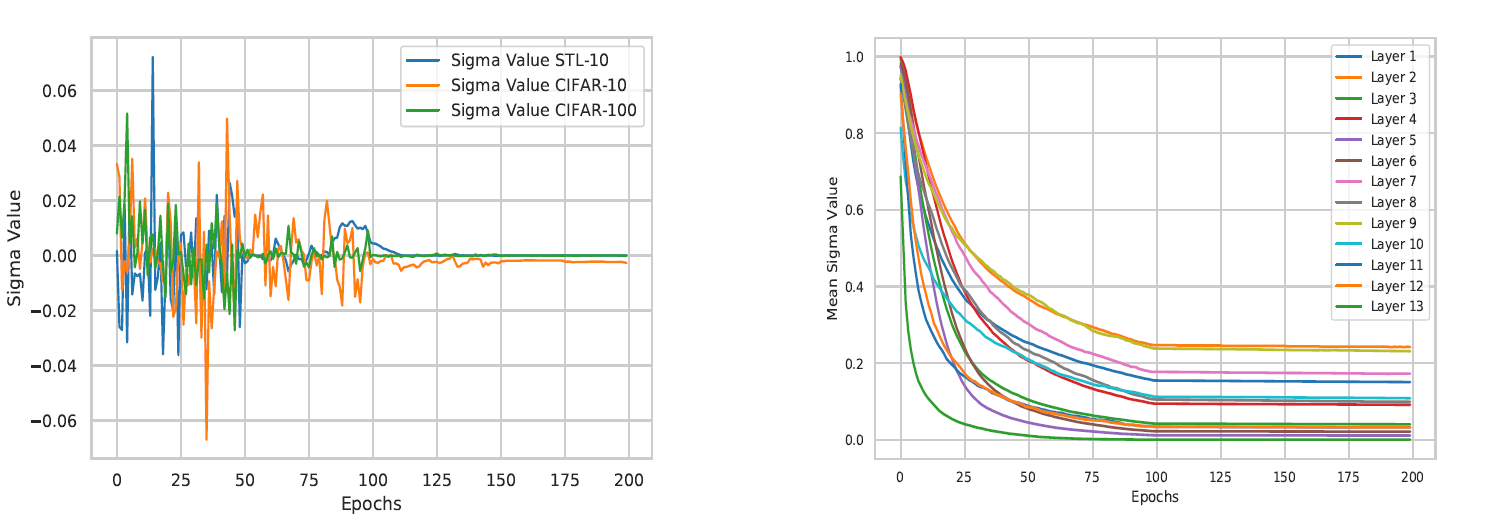
\includegraphics[width=\linewidth]{SigmaTraining.png} 
   \caption{Tratto da \cite{lee2019probact}. A sinistra la transizione del singolo sigma addestrabile nelll'architettura VGG-16 sui tre set di dati. A destra il valore medio dei $\sigma$ addestrati sul set di dati CIFAR10, evidenziando i diversi valori per ogni layer.}
  \label{SigmaTrainingpng}
  \end{figure}

  
  Il training \'e costituito da 400 epochs, ma non vengono mostrati i dati relativi alle epochs superiori a 200 in quanto non hanno contribuito significativamente al training. Infatti gi\'a dopo solo 100 epochs la $single$ $trainable$ $\sigma$ tende a 0. 
  Figura \ref{kFreqDistrpng} mostra la distribuzione in frequenza dell' elemento $k$ dopo 400 epochs. Osserviamo due picchi per ogni distribuzione attraverso i 3 dataset.  
  \begin{figure}[h!]
   \centering
   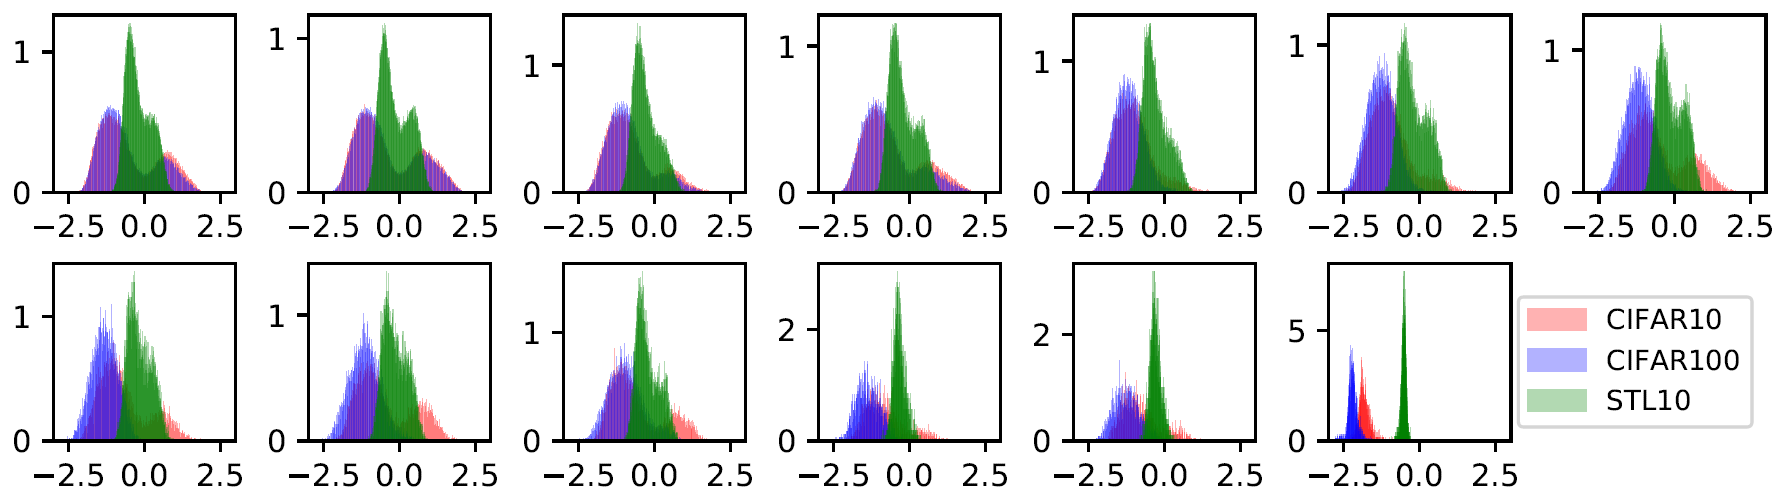
\includegraphics[width=\linewidth]{kFreqDistr.png} 
   \caption{Tratto da \cite{lee2019probact}. Distribuzione in frequenza dell' elemento $k$ dopo l'allenamento dell'architettura VGG-16 per i set di dati CIFAR-10, CIFAR-100 e STL-10 per ogni layer. L'asse X indica il valore $k$ dopo l'allenamento e l'asse Y indica la sua frequenza. Ogni sottofigura rappresenta un layerin cui viene applicata la funzione d'attivazione stocastica, a partire dal primo layer in alto a sinistra fino all'ultimo layer in basso a destra.}
  \label{kFreqDistrpng}
  \end{figure}
  
  Un elevato valore di $\sigma$ agisce come un regolarizzatore interno, migliorando la generalizzazione e prevenendo l'overfitting. Per definire il livello di overfitting di una rete utilizziamo un termine $\gamma$ che mostra la differenza di accuratezza tra training e test:
  \begin{equation}
   \gamma = TrainAccuracy(\%) - TestAccuracy(\%).
  \end{equation}
  
  Se $\gamma$ \'e piccolo, la rete in seguito al training si \'e generalizzata bene anche al set di test. Se invece \'e grande, la rete ha imparato molto bene a classificare gli esempi del training, ma non riesce a classificare casi diversi da quelli gi\'a visti. In figura \ref{WithWithoutDropoutpng} si confrontano le abilit\'a di generalizzazione con e senza l'utlizzo di dropout per il dataset CIFAR-100. 
  \begin{figure}[h!]
   \centering
   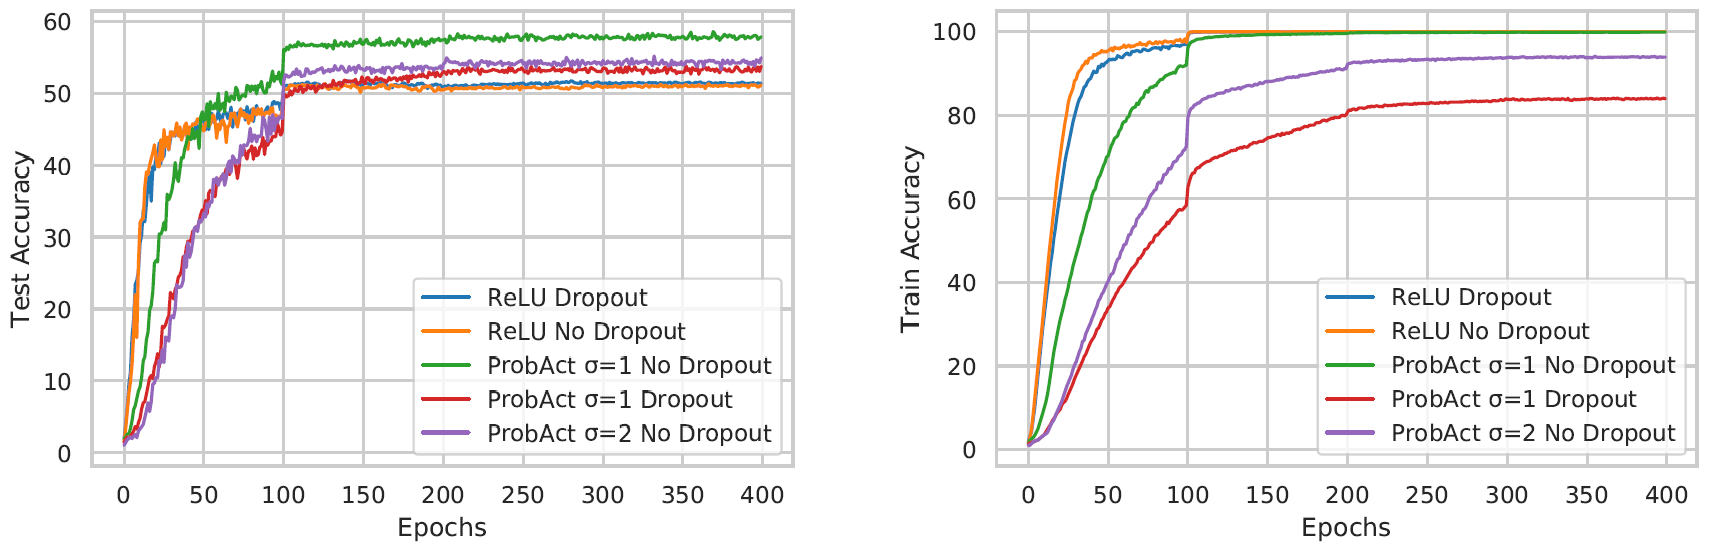
\includegraphics[width=\linewidth]{WithWithoutDropout.png} 
   \caption{Tratto da \cite{lee2019probact}. Confronto tra ReLU e funzione d'attivazione stocastica, sia con che senza dropout, utilizzando il dataset CIFAR-100. In particolare a sinistra il confronto \'e effettuato nel set di test e a destra nel set di training.}
  \label{WithWithoutDropoutpng}
  \end{figure} 
  
  
  Il dropout viene applicato con una probabilit\'a del 0.5\%. La rete senza dropout e con funzione d'attivazione ReLU ha circa $\gamma = 48\%$, valore che non viene modificato di molto se introdotto il dropout. D'altra parte, fissato $\sigma = 1$ si raggiunge $\gamma = 43\%$ e con $\sigma = 2$ si abbassa ulteriormente a $\gamma = 39\%$, sempre senza utilizzare il dropout. Introducendo anche il dropout si ottiene $\gamma = 30\%$ con $\sigma = 1$.
  Una funzione d'attivazione stocastica diventa particolarmente efficace nel caso in cui si abbia un dataset ridotto. Per confermare ci\'o sono stati confrontati i risultati di reti identiche, una con funzione d'attivazione ReLU e l'altra con funzione d'attivazione stocastica (ProbAct \cite{lee2019probact}), utilizzando solo una frazione dei dataset CIFAR-10 e CIFAR-100. I risultati ottenuti sono mostrati in tabella \ref{PartialDatasetTab}.
  \begin{table}[h]\caption{Tratto da \cite{lee2019probact}. Confronto dell'accuratezza del test tra ReLU e ProbAct su sottoinsiemi ridotti di CIFAR-10 e CIFAR-100 (50\% e 25\% del set di dati originale). L'accuratezza del test indicata \'e data dalla media su tre serie di test. Sono stati evidenziati i risultati migliori (tutti appartenenti a ProbAct).} \label{PartialDatasetTab}
   \centering
   \begin{tabular}[h]{|l|c|c|c|c|}
    \hline
    Activation function & CIFAR-10 (50\%) & CIFAR-100 (50\%) & CIFAR-10 (25\%) & CIFAR-100 (25\%) \\ \hline
    ReLU & 82.74\% & 42.36\% & 75.62\% & 30.42\% \\ 
    ProbAct & \textbf{84.73\%} & \textbf{46.11\%} & \textbf{79.02\%} & \textbf{31.67\%} \\ \hline
   \end{tabular}
  \end{table}
 
  
 Questa non \'e che una proposta di applicazione e in generale di studio di reti neurali a valori complessi nel campo del MRF. Le reti neurali presentano ancora margini di miglioramento ed in particolare quelle a valori complessi che fino a non molto tempo fa suscitavano scarso interesse per via delle difficolt\'a di calcolo per la back-propagation. Nel caso in cui effettivamente possano risultare un'alternativa concreta alle tecniche attuali, non solo si riuscirebbero a misurare pi\'u parametri MR contemporaneamente, ma si potrebbe avere un riscontro quasi immediato e di tipo quantitativo.
 
 
 \chapter*{Applicazione delle reti neurali al problema del MRF}\label{MRIsection}
 
 Le reti neurali a valori complessi sembrano essere pi\'u performanti rispetto a quelle reali nel caso l'input da analizzare sia naturalmente esprimibile nel campo complesso \ref{CompR-Csection}. Per questo motivo si \'e scelto di studiare in parallelo ai possibili vantaggi e svantaggi della rete neurale a valori complessi, una possibile applicazione nel campo della risonanza magnetica, in particolare nel MRI fingerprinting.
 
 \section{MRF con reti neurali a valori reali}
 
 Recentemente il MRF \'e stato proposto come tecnica di imaging quantitativa per l'acquisizione simultanea di parametri tissutali come i tempi di rilassamento T1 e T2. Sebbene l'acquisizione sia altamente accelerata, la ricostruzione soffre di lunghi tempi di calcolo: i metodi di matching usati per trovare il segnale pi\'u simile a quello misurato devono confrontare quest'ultimo con un numero elevato di segnali simulati. Gli approcci di deep-learning possono superare questa limitazione, fornendo la mappatura diretta dal segnale misurato attraverso una rete neurale. 
 
 Per evitare errori o imprecisioni, il dizionario viene in genere calcolato con una granularit\'a fine su una gamma molto vasta di possibili valori dei tessuti. Le dimensioni del dizionario tuttavia, aumentano in modo esponenziale all'aumentare del numero di parametri tissutali, il che pu\'o rapidamente portare a dizionari proibitivi di grandi dimensioni, che richiedono ingenti risorse di elaborazione. Questo aumento della memoria, dell'archiviazione e dell'onere computazionale \'e un fattore limitante per l'adozione clinica dei metodi MRF. Ridurre la densit\'a del dizionario come proposto in precedenza, non \'e per\'o una soluzione convincente a questo problema perch\'e limita a priori l'accuratezza della ricostruzione, senza considerare ancora imprecisioni dovute a fattori sperimentali. 
 
 Il lavoro matematico nella teoria delle reti neurali e algoritmi di deep-learning ha dimostrato che qualsiasi funzione di Borel pu\'o essere rappresentata da una rete neurale con un numero finito di neuroni, che possono quindi offrire una rappresentazione compatta di funzioni complicate \cite{hornik1989multilayer}. Sfruttando questa propriet\'a si pu\'o cercare una rete neurale che sfrutti il dizionario come set di training e/o set di test e che vada a sostituire il lento processo di matching, infatti in termini di spazio di archiviazione sarebbe pi\'u compatta di un dizionario ed il processo di matching, una volta compiuto il training verrebbe drasticamente velocizzato.
 
 Per verificare l'efficienza di questo modello, in \cite{cohen2018mr} viene definita una rete neurale con 4 layer (uno di input, 2 hidden layer e un layer di output) utilizzando il TensorFlow \cite{abadi2016tensorflow}. L'input consiste di 25 o 50 nodi e l'output da 2 nodi in quanto sono studiati solo il T1 e il T2. Ogni hidden layer \'e composto da 300 nodi. Le dimensioni della rete sono state selezionate empiricamente, cercando un buon compromesso tra il tempo di addestramento della rete, lo spazio di archiviazione e l'accuratezza delle ricostruzioni. Il tasso di apprendimento della rete \'e stato impostato come 0.001 e la funzione di costo \'e data dall'errore quadratico medio. Il training viene effettuato sfruttando un dizionario con circa 69000 esempi, mentre per la convalida \'e stato sfruttato il BrainWeb digital brain phantom insieme a simulazioni montecarlo, introducendo rumore  gaussiano. L'accuratezza della rete \'e comparabile a quella dei metodi tradizionali di MRF e in particolare \'e stato riscontrato una migliore efficienza in caso di rumore o undersampling.
 
 
 
 \section{MRF con reti neurali a valori complessi}
 
 Dati i risultati ottenuti con le reti neurali a valori reali (gi\'a promettenti) e i miglioramenti ottenuti dalle reti neurali a valori complessi nell'analisi di segnali ondulatori nei confronti delle reti a valori reali, propongo in questo documento l'applicazione di queste ultime al problema MRF.
 
 L'argomento \'e stato trattato anche in \cite{virtue2017better}, dove si comparano diversi metodi applicabili al fingerprinting. Riportiamo di seguito i metodi comparati ed i risultati ottenuti:
 \begin{itemize}
  \item prodotto scalare del segnale misurato con quello simulato del dizionario;
  \item rete neurale a 2 canali, che lavorano separatamente su parte reale e parte immaginaria del segnale;
  \item rete neurale a valore reale analoga alla precedente, ma di dimensione doppia, con 1024 e 512 `` feature channels'' nei 2 hidden layer;
  \item rete neurale a valori complessi, con un solo canale che utilizza la ``cardioid activation function'' definita nel documento citato;
  \item rete neurale a valori complessi che utilizza come funzione di attivazione una sigmoide applicata separatamente a parte reale e parte immaginaria;
  \item rete neurale a valori complessi che utilizza la funzione d'attivazione siglog \cite{georgiou1992complex};
 \end{itemize}

 Come risultato in \cite{virtue2017better} si ottiene che le reti neurali in generale sono pi\'u efficaci nella predizione dei valori T1 e T2, mentre il prodotto scalare rimane il pi\'u accurato per quanto riguarda $\Delta\mbox{B}_0$. Nel confronto tra reti neurali a valori reali e reti a valori complessi, queste ultime sembrano performare meglio. In particolare nel caso di segnale pulito, la rete a valori complessi prevale in accuratezza sia su T1 che su T2, mentre prevale solo nell'accuratezza su T1 in caso di segnale con rumore.

 
 \chapter*{Conclusioni}
 
 La risonanza magnetica si \'e dimostrata estremamente utile per la diagnosi, la prognosi e la valutazione terapeutica, ma ha lo svantaggio di essere lenta rispetto ad altri strumenti diagnostici. 
 Inoltre \'e generalmente qualitativa: il principale mezzo di informazione utilizzato per caratterizzare una patologia \'e il contrasto tra i tessuti.
 
 Si cerca di sopperire alla mancanza di misure oggettive attraverso il MRF, tecnica di risonanza magnetica quantitativa che presenta una notevole velocizzazione nell'acquisizione del segnale, con il vantaggio di ottenere da questo i valori di pi\'u di un parametro per volta, ma con lo svantaggio principale di spendere molto tempo nel matching tra segnale e dizionario.
 
 Le reti neurali sembrano essere una soluzione efficace: velocizzano i tempi di calcolo dei parametri da studiare e non necessitano della creazione del dizionario per ogni acquisizione perch\'e capaci di generalizzazione. 
 In particolare quelle a valori complessi sembrano essere maggiormente efficienti se l'input \'e di natura ondulatoria, proprio come nel caso della risonanza magnetica.
 
 Il loro utilizzo per\'o non \'e ancora popolare e gli accorgimenti necessari per il loro funzionamento non sono banali, a partire dalla derivazione della funzione di costo.
 Per questo motivo \'e difficile garantire il successo di tali modelli che, per l'appunto, non sono ancora utilizzati in ambito clinico.
 A questo proposito sono state discusse anche tecniche di ottimizzazione e generalizzazione delle reti neurali, da applicare assieme alle reti neurali a valori complessi, come gli ensemble di reti e la funzione d'attivazione stocastica.
 Tutto ci\'o nella speranza che questa possa effettivamente essere una risposta concreta al problema del MRF affrontato.
 
 \bibliographystyle{unsrt}
 \bibliography{bibliografia}
 
\end{document}
